\documentclass[12pt,a4paper]{report}

% , Page geometry (standard 25 mm margins) , 
\usepackage[a4paper,margin=25mm]{geometry}

% , Fonts: Times-equivalent (newtx unavailable; mathptmx provides Times text + math) , 
\usepackage[T1]{fontenc}
\usepackage[utf8]{inputenc}
\usepackage{mathptmx}
\usepackage{textcomp}

% , Maths, graphics, tables , 
\usepackage{amsmath,amssymb}
\usepackage{graphicx}
\graphicspath{{./}}
\usepackage{booktabs}
\usepackage{array}
\usepackage{caption}
\captionsetup{font=small,labelfont=bf}

% , Spacing and headings , 
\usepackage{setspace}
\onehalfspacing
\usepackage{titlesec}
% Chapter format: "N | Title"
\titleformat{\chapter}[hang]
  {\normalfont\Huge\bfseries}{\thechapter\,\,\textbar}{0.4em}{}
\titlespacing*{\chapter}{0pt}{10pt}{30pt}

% , Citations: Harvard / author-date , 
\usepackage[round,authoryear]{natbib}
\bibliographystyle{apalike}
\setcitestyle{aysep={}}

\usepackage[hidelinks]{hyperref}
\usepackage{xurl}

\title{Between Culture and Cost}
\author{Roudra Sarkar}
\date{10 August 2026}

\begin{document}

% ==========================================================================
% TITLE PAGE
% ==========================================================================
\begin{titlepage}
\centering
\vspace*{2.5cm}
{\LARGE\bfseries Between Culture and Cost\par}
\vspace{0.6cm}
{\large Mechanisms of the education--fertility gradient across Europe and a British cohort\par}
\vfill
{\large Roudra Sarkar\par}
\vspace{1.4cm}
{\normalsize MSc Dissertation submitted in partial fulfilment of the requirements\\
for the degree of MSc in Applied Social Data Science\par}
\vspace{1.0cm}
{\normalsize School of Social Sciences and Philosophy\\
Department of Political Science\par}
\vspace{1.0cm}
{\normalsize Supervisor: Dr Thomas Chadefaux\par}
\vspace{1.4cm}
{\normalsize Trinity College Dublin\par}
\vspace{0.4cm}
{\normalsize 10 August 2026\par}
\vfill
{\footnotesize Note: Student ID is intentionally not printed (university guidance).\par}
\end{titlepage}

\pagenumbering{roman}

% ==========================================================================
% DECLARATION
% ==========================================================================
\chapter*{Declaration}
\addcontentsline{toc}{chapter}{Declaration}
I hereby declare that this MSc Dissertation is entirely my own work and that it has not
been submitted as an exercise for a degree at this or any other university. I have read
and I understand the plagiarism provisions in the General Regulations of the University
Calendar for the current year, found at \url{http://www.tcd.ie/calendar}. I have also
completed the Online Tutorial on avoiding plagiarism ``Ready Steady Write'', located at
\url{http://tcd-ie.libguides.com/plagiarism/ready-steady-write}.

\vspace{1.5cm}
\noindent Signed: \rule{6cm}{0.4pt}

\vspace{0.8cm}
\noindent Date: \rule{6cm}{0.4pt}

% ==========================================================================
% ABSTRACT
% ==========================================================================
\chapter*{Abstract}
\addcontentsline{toc}{chapter}{Abstract}
This dissertation asks what shape the education--fertility gradient takes across European
populations in the period 2007--2024, and what conditions predict its steepness, its shape,
and the individual-level mechanism through which it operates. The demographic transition
fitness paradox, that resources and reproduction, historically positively coupled, now
co-vary negatively in high-income societies, is tested through four hypotheses that
discriminate between cultural-transmission, quantity--quality, and maladaptation accounts.
I assemble an unbalanced country--year--education panel of period education-stratified
total fertility rates for 21 European countries from Eurostat, a country-level cross-section
combining institutional (V-Dem), attitudinal (European Social Survey), and economic
predictors, and an individual-level sample from the 1970 British Cohort Study. Methods are
matched to scale: two-way fixed-effects, quadratic, and quantile regression for the
population gradient; a two-stage XGBoost--SHAP discovery and Bayesian-inference pipeline for
cross-country variation; and double machine learning causal mediation for the individual
mechanism. The central finding is that the contemporary European gradient is not a monotonic
relationship in quantum but a U-shape in level combined with a tempo effect concentrated in the early
twenties. Medium-educated women record the lowest fertility in fourteen of twenty-one
countries, confirming both a negative low--high contrast (H1) and non-monotonicity (H2). The H1
contrast is a phenomenon of timing rather than quantum: it is located
entirely in ages 20--24 and reverses when the rate is computed over ages 25--49, whereas
medium-educated women record the lowest fertility at every age floor, though which arm of the
U is statistically identified depends on the specification. At
the country level (H3), neither cultural nor economic indicators dominate at this sample
size, with GDP per capita the most precisely identified single predictor. At the individual
level (H4), the mechanism is economic rather than attitudinal: earnings account for
between two-fifths and three-fifths of the education effect on women's fertility, depending on whether
sample composition is held fixed, while the attitudinal pathway is negligible and its sign is unstable
across specifications. This reverses the hypothesised ordering.
The contemporary paradox is therefore
narrower, and more economically rational at the proximate level, than the classical framing
implied.

% ==========================================================================
% ACKNOWLEDGEMENTS
% ==========================================================================
\chapter*{Acknowledgements}
\addcontentsline{toc}{chapter}{Acknowledgements}
% [Placeholder, personalise before submission.]
I would like to thank my supervisor, Dr Thomas Chadefaux, for guidance throughout this
dissertation, and the MSc in Applied Social Data Science teaching team for their
methodological training and support.

% ==========================================================================
% CONTENTS
% ==========================================================================
\tableofcontents
\listoffigures
\listoftables

\clearpage
\pagenumbering{arabic}

% ==========================================================================
% CHAPTER 1
% ==========================================================================
\chapter{Introduction}

\section{Background and motivation}
Across most of human history, socioeconomic resources and reproductive success co-varied
positively: those with greater access to land, livestock, or social standing produced more
surviving offspring \citep{boone1986,voland1990,hopcroft2006,nettlepollet2008}. The demographic
transition of the eighteenth and nineteenth centuries decoupled and often inverted this
relationship, so that in contemporary high-income societies those with the highest education
and income tend to have the fewest children. \citet{vining1986} named this the central
theoretical problem of human sociobiology, and four decades on its mechanisms remain
contested.

Three families of explanation compete, cultural transmission, the quantity--quality tradeoff, and
evolutionary maladaptation (Chapter~2), making different predictions about where the gradient should
appear and steepen. A
more recent literature questions whether the gradient is uniformly negative: \citet{hopcroft2006}
and others report fertility rising with income among men, and a broader pattern of the relationship
ceasing to decline at the top of the distribution, a J-curve, consolidated in the review by
\citet{stulpbarrett2016}. If genuine, the paradox may be narrower than first framed, but the evidence
is methodologically uneven: few studies
use education-stratified fertility across multiple countries, and modern distributional methods
are rarely deployed.

\section{Research problem and question}
The literature suffers three interlocking gaps. First, systematic multi-country tests of the
J-curve using education-stratified fertility are lacking; existing evidence is fragmentary and
rarely uses formal distributional methods. Second, cross-country comparisons of cultural and
economic mechanisms rely on small numbers of pre-selected covariates in low-sample country-level
regressions, vulnerable to omitted-variable bias and overfitting. Third, individual-level
mediation analyses of the education effect rarely use modern methods for high-dimensional
confounding. The 1970 British Cohort Study (BCS70), whose Age 51 sweep now provides essentially
complete fertility, remains underused for this question. I therefore ask: across European
populations, what is the shape of the contemporary education--fertility gradient, and what
conditions predict its steepness and the location of any non-monotonicities?

\section{Hypotheses}
The question decomposes into four hypotheses, each anchored to a theoretical source.

\textit{H1 (Inversion).} Across European populations observed between 2007 and 2024, the
relationship between education and period fertility is negative, after controlling for
country- and year-specific factors, the descriptive claim that motivates the paradox
\citep{vining1986}.

\textit{H2 (Non-monotonicity).} The relationship is non-monotonic, with period fertility ceasing to
decline, or rising, at the upper end of the educational distribution, the J-curve revival
\citep{stulpbarrett2016}, of which the positive male income--fertility gradient of
\citet{hopcroft2006} is a cognate finding.

\textit{H3 (Cultural transmission).} Cross-country variation in the steepness and shape of the
gradient is predicted better by cultural indicators (secularisation, individualism, gender-norm
change) than by economic indicators (GDP per capita, female labour-force participation,
contraceptive prevalence), the country-level prediction of cultural-transmission theory
\citep{bongaartswatkins1996,colleran2016}.

\textit{H4 (Individual mechanism).} Within BCS70 individuals, the effect of education on
completed fertility is mediated primarily by attitudinal and preference variables rather than
by realised earnings, the individual-level prediction of the same theory, and a test of whether the
persistent direct education effect reported by \citet{snopkowski2016} operates through attitudinal
channels in an industrialised setting.

The hypotheses discriminate between the three frameworks rather than confirming any one. A pattern in
which the gradient is non-monotonic (H2), cultural indicators dominate cross-country variation (H3), and
attitudinal pathways dominate individual mediation (H4) would constitute strong evidence for cultural
transmission; the opposite pattern would favour quantity--quality.

\section{Contribution}
I make three substantive contributions. First, a methodologically modern multi-country test of
non-monotonicity, using both parametric (quadratic fixed-effects) and semi-parametric (quantile)
methods across 21 European countries, going beyond the single-country, single-method designs that
have characterised the J-curve literature. Second, a principled high-dimensional comparison of
cultural and economic explanations of cross-country variation, combining gradient-boosted
variable importance (XGBoost with SHAP values) with Bayesian regression in an
exploratory-then-confirmatory pipeline that separates discovery from inference. Third, an
individual-level mediation analysis using double
machine learning \citep{chernozhukov2018} on the BCS70 cohort, whose age-42 fertility outcome
can now be validated as essentially complete by the recently released Age~51 sweep.

\section{Findings in brief}
The four hypotheses receive heterogeneous support. The gradient is U-shaped rather than
monotonic: medium-educated women record the lowest fertility in fourteen of twenty-one countries, with
both low- and high-educated women higher. The high--low contrast is negative on average, supporting H1,
but this contrast is a phenomenon of fertility timing: it is concentrated entirely in ages 20--24 and
reverses once the rate is computed over ages 25--49. The strict monotonic prediction is rejected in the
great majority of countries, so H2 is confirmed in a stronger form than originally specified. H3
produces no clear winner, SHAP importance slightly favours cultural predictors, the Bayesian
comparison an economic model, with substantial uncertainty at 21 countries, while H4 is the most
surprising result: contrary to the hypothesis, earnings account for the majority of the education
effect and attitudes contribute little, favouring quantity--quality over cultural transmission at the
individual level. Table~\ref{tab:hypsummary} summarises the four hypotheses, their tests, and their
verdicts. Chapter~2 reviews the literature; Chapter~3 sets out data and methods; Chapters~4--6
report the descriptive, main, and mechanism results; and Chapters~7--8 discuss and conclude.

\begin{table}[ht]
\centering
\caption{The four hypotheses: prediction, test, principal result, and verdict.}
\label{tab:hypsummary}
\small
\begin{tabular}{@{}p{0.10\textwidth}p{0.20\textwidth}p{0.20\textwidth}p{0.24\textwidth}p{0.14\textwidth}@{}}
\toprule
& Prediction & Test & Principal result & Verdict \\
\midrule
H1 & Education and fertility negatively related & Two-way FE on 21-country eTFR panel & High vs low $\beta=-0.187$ ($p=0.002$); reverses to $+0.201$ over ages 25--49 & Supported, but a tempo effect \\
H2 & Relationship non-monotonic at the top & Quadratic and quantile FE regression & $\beta_2=+0.195$ ($p<0.001$); medium lowest in 14 of 21 countries & Supported \\
H3 & Cultural indicators predict cross-country variation better than economic & XGBoost--SHAP then Bayesian model comparison, $N=21$ & LOOCV $R^2=-0.086$; SHAP favours cultural, WAIC favours economic; all intervals cross zero & Unsupported at this sample size \\
H4 & Education effect mediated by attitudes rather than earnings & DML mediation on BCS70, $N=1{,}461$ women & Earnings 44--61\% of total effect; attitudinal share negligible and sign-unstable & Falsified \\
\bottomrule
\end{tabular}
\end{table}

% ==========================================================================
% CHAPTER 2
% ==========================================================================
\chapter{Literature Review}

\section{The paradox and the demographic transition}
The demographic transition fitness paradox is the observation that, in contemporary
high-income populations, individuals with greater socioeconomic resources tend to produce
fewer offspring than those with fewer resources, directly contradicting the evolutionary
prediction that organisms convert resources into reproduction. \citet{vining1986} first framed
it as the central theoretical problem of human sociobiology, and nearly four decades on it
remains unresolved across evolutionary anthropology, behavioural ecology, formal demography,
sociology, and economics.

The demographic transition is the historical shift from high fertility and mortality to low
\citep{notestein1945,caldwell1976}. Across pre-transition agrarian populations the
wealth--reproduction relationship was typically positive: wealthier landholders and
higher-ranking nobles had more surviving children \citep{boone1986,voland1990,pettay2005}, a
pattern that reviews suggest dominated prior to industrialisation
\citep{hopcroft2006,nettlepollet2008}. The reversal occurred unevenly across Europe, earlier in
Sweden and Britain, later in the south and east \citep{dribe2014,goodman2012,colemansalt1992}. By the
mid-twentieth century the negative gradient was a defining feature of fertility across the
developed world and has persisted, with considerable variation in magnitude and shape
\citep{skirbekk2008,andersson2009}. It was not anticipated by classical transition
theory \citep{mason1997}; \citet{vining1986} pointed out that no equivalent reversal had been
documented in any other species, so the human pattern requires a specifically human explanation.

\section{Theoretical explanations}
Three frameworks dominate. They are not mutually exclusive, but they make different predictions
about where the gradient should appear and steepen.

\subsection{Cultural transmission}
The cultural-transmission framework argues that the transition propagates not through individual
responses to changed economic conditions but through the social learning of low-fertility norms,
typically from higher- to lower-status individuals \citep{bongaartswatkins1996}.
\citet{bongaartswatkins1996} showed that the timing of fertility decline across 69 countries was
poorly predicted by economic indicators alone but well predicted by indicators of social
interaction. Cultural-evolutionary theory formalises this, modelling fertility norms as
transmissible traits subject to prestige and conformity biases \citep{boydricherson1985,mesoudi2011}.
The most influential ideational account is the Second Demographic Transition framework, which
attributes late-modern demographic change to a value shift toward self-realisation and individual
autonomy. \citet{lesthaeghe2010} traces its spread across
European populations and argues that cross-national differences in period fertility have been
driven largely by differential rates of postponement and recuperation, a point that
anticipates the tempo findings of Chapter~5; it is also the tradition from which the attitudinal
predictors used for H3 and H4 are drawn.
\citet{colleran2016,colleran2020} argues that the cultural account explains features economic
accounts struggle with, among them the rapidity of decline and the persistence of
low fertility after the conditions that favoured it have changed, with support from the
geographical and network clustering of fertility behaviour \citep{watkins1991,balbobarban2014} and
from agent-based simulations \citep{colleranmace2015}.
The framework predicts that cross-country variation in the timing of inversion should be predicted
by indicators of cultural transmission rather than by economic indicators alone, the prediction
tested as H3.

\subsection{Quantity--quality tradeoff and embodied capital}
The quantity--quality framework, originating in \citet{becker1960} and developed for evolutionary
purposes by \citet{kaplan1996} and \citet{kaplanlancaster2003}, argues that high returns to human
capital give modern parents an unprecedented incentive to substitute investment per child for
number of children. \citet{lawsonmace2011} support this with sibling-competition evidence: children
in larger families show reduced cognitive, educational, and health outcomes. The principal challenge
is empirical: \citet{goodman2012}, using multigenerational Swedish data, found that low fertility
increases descendant socioeconomic position but does not maximise long-run reproductive
success, larger families produce more grandchildren on average, implying that if quantity--quality
substitution occurs it is not actually maximising biological fitness.

\subsection{Maladaptation and evolutionary lag}
A third framework treats modern low fertility as a maladaptive response to evolutionary novelty:
the psychological mechanisms that historically converted resources into reproduction are not
well calibrated to contraception, extended education, and welfare provision
\citep{perusse1993,kanazawa2003}. It is often invoked descriptively rather than tested, and sits
uneasily with evidence that fertility responds to current economic conditions \citep{sobotka2011};
it is best understood as complementary to the cultural and economic accounts.

\section{The J-curve and recent developments}
A more recent literature questions the assumption of a uniformly negative gradient.
\citet{hopcroft2006}, analysing biological-children counts for a US probability sample, finds a
positive income--fertility gradient among men even as education, occupation, and other status
measures depress fertility for both sexes; she attributes the conventional negative gradient partly
to standard status categories pooling men and women, and to income and intelligence exerting
opposing effects. \citet{fiederhuber2007} found analogous
patterns among Swedish men. \citet{stulpbarrett2016} provide the most systematic review,
concluding that the relationship is heterogeneous across populations, sub-groups, and periods,
and that whether the modern relationship is a paradox depends on which sub-population and fertility
measure is examined. If fertility revives at the top of the distribution, the paradox may be more
limited, affecting the middle but not the extremes, implying that the psychology of
resource-to-fertility conversion is partially intact. The J-curve literature nonetheless remains
methodologically uneven: few studies use education-stratified fertility across multiple countries,
and quantile or spline methods are rare, leaving cross-national robustness unsettled. The closest
existing comparison is \citet{jalovaara2019}, who use harmonised Nordic register data to measure
completed cohort fertility and childlessness by education and sex. They find that women's negative
educational gradient in completed fertility has \emph{vanished} in Denmark, Norway and Sweden, though
not in Finland, while men's positive gradient persists and low-educated men retain both the lowest
fertility and the highest childlessness. Childlessness among women has reversed its gradient
entirely: highest among the highly educated in the 1940s cohorts, it is now highest among the least
educated. They attribute this to the growing social and economic marginalisation of a shrinking
low-education segment. Their cohort measure is superior to the period rates used here, and their
Nordic findings converge with the flat and inverted gradients this dissertation recovers for Denmark,
Norway and Sweden, which is reassuring for the descriptive results even though the measures differ.

\section{Individual-level mechanism studies}
A smaller literature examines the pathways by which education depresses fertility.
\citet{skirbekk2008} identifies three: an enrolment effect (extended schooling postpones
childbearing); an opportunity-cost effect (higher education raises the wage cost of childrearing);
and a preference effect (education changes values on gender roles, autonomy, and ideal family
size). Disentangling them is demanding because education is endogenous; quasi-experimental studies
using compulsory-schooling reforms find exogenous education effects smaller than cross-sectional
associations imply and operating mainly on timing \citep{monstad2008,cyganrehm2013}.
\citet{snopkowski2016}, using structural equation models across three populations, found that
education retains a direct effect on fertility in two of their three sites even after controlling for
a range of economic and cultural-transmission mediators (women's work, husband's education, local
mortality, social networks, and contraceptive knowledge and use); the authors are agnostic about this
residual, suggesting it may reflect horizontal cultural transmission or unobserved characteristics of
particular contexts. Their finding that a direct education effect can persist beyond measured
mediators motivates the individual-level decomposition in H4. The British cohort studies have been used
extensively in adjacent work: \citet{berrington2017} used BCS70 to show that delayed childbearing
increasingly resulted in unintended childlessness for highly educated women, but formal mediation
analyses separating economic from attitudinal pathways with modern causal-inference methods remain
rare.

\section{Gaps and contribution}
Three gaps motivate this dissertation. First, systematic multi-country tests of the J-curve using
education-stratified fertility and formal distributional methods are lacking. Second, cross-country
work tends to use few pre-selected covariates in small-sample regressions that risk both
omitted-variable bias and overfitting; a principled high-dimensional analysis combining regularised
machine learning with interpretable variable importance \citep{atheywager2019,lundberglee2017} and
formal Bayesian estimation would be an advance. Third, individual-level mediation has rarely been
subjected to formal causal mediation with modern adjustment for high-dimensional confounding
\citep{chernozhukov2018}; the BCS70, with rich attitudinal and economic measures and a recently
released Age 51 sweep, is well suited but has not, to my knowledge, been used for this purpose. H1
and H2 establish and formally test the descriptive pattern; H3 compares cultural and economic
explanations of cross-country variation; and H4 decomposes the individual education effect. Together
they offer a more rigorous and theoretically integrated account of the contemporary gradient than
has hitherto been available.

% ==========================================================================
% CHAPTER 3
% ==========================================================================
\chapter{Data and Methodology}

\section{Research design}
The empirical strategy tests each hypothesis at the scale at which it makes its claim, moving from
macro to micro with a method matched to each data structure. Three analytical datasets are
constructed. Dataset~1 is an unbalanced country--year--education panel of period total fertility
rates for 21 European countries, 2007--2024 (933 observations), used for H1 and H2. Dataset~2 is a
country-level cross-section of 21 observations combining derived gradient outcomes with cultural,
economic, and regional predictors, used for H3. Dataset~3 is the individual-level sample from the
1970 British Cohort Study, used for H4. Table~\ref{tab:datasources} summarises the sources \citep{eurostat_faeduc,eurostat_edat,vdem2026,ess2024,oecd_gdp,oecd_lfp,worldbank_contra,bcs70_birth,bcs70_age42,bcs70_age51}.

\begin{table}[ht]
\centering
\caption{Data sources.}
\label{tab:datasources}
\footnotesize
\resizebox{\textwidth}{!}{%
\begin{tabular}{@{}llll@{}}
\toprule
Source & Unit & Coverage & Role \\
\midrule
Eurostat \texttt{demo\_faeduc} & Country $\times$ year $\times$ age $\times$ ISCED & 21 countries, 2007--2024 & Births numerator (H1, H2) \\
Eurostat \texttt{edat\_lfse\_03} & Country $\times$ year $\times$ age $\times$ ISCED $\times$ sex & 21 countries, 2007--2024 & Education shares (H1, H2) \\
Eurostat \texttt{demo\_pjangroup} & Country $\times$ year $\times$ age $\times$ sex & 21 countries, 2007--2024 & Population denominator (H1, H2) \\
V-Dem v16 & Country $\times$ year & 21 countries, 2007--2024 & Institutional predictors (H3) \\
OECD & Country $\times$ year & 18--19 of 21 & Economic predictors (H3) \\
World Bank & Country $\times$ year & 12 of 21 & Contraceptive prevalence (H3) \\
ESS rounds 1--11 & Individual, pooled & 19--20 of 21 & Attitudinal predictors (H3) \\
BCS70 (UK Data Service) & Individual, longitudinal & $\approx$17{,}000, sweeps to age 51 & Individual mediation (H4) \\
\bottomrule
\end{tabular}%
}
\end{table}

The strategy diverges from the original proposal in three respects. First, the primary outcome is
period education-stratified TFR (eTFR) from Eurostat rather than completed cohort fertility from the
Wittgenstein Centre, whose R interface exposes only projection data (2020--2100), not the historical
reconstruction the proposal assumed; the shift also makes the ESS attitudinal aggregates
contemporaneous with the fertility they explain. Second, the cross-country
sample is 21 rather than the 35 projected, owing to country-specific gaps in Eurostat's
education-stratified reporting. Third, H3 originally relied on five V-Dem institutional indices as
cultural predictors; these proved to measure institutional quality rather than
individual attitudes, so three attitudinal composites from eight ESS core-module items
were added alongside them. All three departures
reflect data availability or analytical refinement, not results-driven choices.

\section{Dataset 1: education-stratified period fertility}
\label{sec:etfr}
Three Eurostat series form the backbone. \texttt{demo\_faeduc} provides live births by mother's
five-year age group and ISCED 2011 attainment; \texttt{edat\_lfse\_03} provides the educational
composition of the female population; and \texttt{demo\_pjangroup} provides total female population
by five-year age group. Education-specific female population in each cell is estimated by
multiplying total population by the education share, under the standard demographic assumption
that educational composition is approximately uniform within five-year subgroups of the wider
reporting bands. That assumption is defensible above age 25, where attainment has largely stabilised,
but weaker at 15--19 and 20--24 where education is still in progress and the
low-education share is mechanically inflated; because those cells contribute
disproportionately to low-tier eTFR, Section~\ref{sec:agefloor} reports an age-floor sweep. The country sample
was the intersection of \texttt{demo\_faeduc} and \texttt{edat\_lfse\_03} after excluding aggregate
units, walking down from an initial 35 to a final 21: twelve countries report fertility only as
``All ISCED levels'', and Bosnia and Herzegovina and Montenegro were dropped for missing population
data and zero year overlap respectively. The United Kingdom is excluded from H1--H3 owing to
post-Brexit reporting gaps but enters through BCS70 in H4. All exclusions reflect
data availability, not analytical choice.

Educational attainment is harmonised to three ISCED 2011 tiers: low (0--2), medium (3--4), and
high (5--8), the most granular grouping jointly available across all 21 countries \citep{skirbekk2008}.
Education-specific age-specific fertility rates (ASFR) are the ratio of births to estimated female
population in each country $\times$ year $\times$ age $\times$ education cell, and the eTFR is
$\mathrm{eTFR}_{r}=5\times\sum_{a}\mathrm{ASFR}_{r,a}$ across the seven five-year age groups spanning
15--49. Numerator and denominator come from different
instruments, a measurement asymmetry that bears directly on the low tier: births are
drawn from vital registration, which is close to complete, while the education denominator is
survey-based, from the Labour Force Survey. Labour force surveys typically under-cover the
least-educated, and any such shortfall makes the low-education denominator too small and the low-tier
eTFR correspondingly too high. This is an alternative reading of the most extreme low-tier values:
Slovakia's mean low-tier eTFR of 2.79 on a low-education share of 6.6\% is what
denominator under-coverage would produce, as well as what over-representation of high-fertility
minority populations would produce, and the two cannot be separated with these data. In 44 high-tier
country--years the 15--19 cell has no usable rate, the tertiary-educated population at that age being
zero or unreported, so the eTFR there is summed over six age groups; since the
15--19 contribution to high-tier fertility is negligible (Section~5.7), this does not
materially affect the rate. The resulting panel comprises 933 observations, unbalanced
within 2007--2024: coverage runs the full window for eight countries but is shorter and
period-specific for the rest, from six years for Austria (2007--2012) to eight for Latvia
(2017--2024). Country and year fixed effects absorb this for H1 and H2; its implication for the
H3 outcome is noted in Section~7.3.

Each country is classified into one of four shape categories from mean eTFR by tier. The primary
distinction is whether medium is the lowest tier (medium~$<$~low and medium~$<$~high). Countries where
it is form the two U-shape categories, split by the share of women aged 25--39 in the low tier:
\emph{composition-driven U-shape} (eight; share $<12\%$) and \emph{broad U-shape} (six; share
$\geq 12\%$). Of the remainder, those with low~$>$~medium~$>$~high are \emph{monotonic negative} (five),
and the residual cases are \emph{inverted bottom} (two). The 12\% threshold sits at a gap in the
distribution of the low-education share, separating a compressed cluster of nine countries below 11\%
from a dispersed remainder above 12.8\%. The cut is pragmatic rather than natural, but it does separate
countries where a small low tier plausibly reflects either minority over-representation or denominator
under-coverage from those where elevated low-tier fertility is structural; the substantive findings are
robust to its value.

\section{Dataset 2: country-level outcomes and predictors}
The primary outcome, \texttt{gradient\_steepness}, is mean $\mathrm{eTFR}_{\text{low}}$ minus mean
$\mathrm{eTFR}_{\text{high}}$ across 2007--2024; positive values denote the conventional negative
gradient. A binary \texttt{u\_shape} flags whether medium is below both other tiers. Cultural
predictors come from two sources operationalising distinct dimensions. V-Dem v16 supplies five
institutional indices (liberal democracy, women's political empowerment, freedom of religion,
electoral and egalitarian democracy), capturing formal institutional structure rather than
individual beliefs; because three of these correlate above $r=0.98$, each Bayesian model includes
at most two. The ESS (rounds 1--11) supplies three attitudinal composites, secularisation,
gender egalitarianism, and an autonomy-versus-conformity index, operationalising the individual
attitudes that cultural-transmission theory identifies as the proximate channels of norm diffusion
\citep{bongaartswatkins1996,colleran2016}. The combination lets H3 distinguish culture operating
through institutions from culture operating through attitudes, a distinction not previously tested
in this literature.

Economic predictors are GDP per capita (OECD, 18 of 21), female labour-force participation (OECD,
19 of 21), and modern contraceptive prevalence (World Bank, 12 of 21). A regional indicator,
\texttt{post\_socialist}, takes the value one for formerly socialist Eastern European states. This
binary necessarily collapses substantial heterogeneity in pronatalist-policy histories across these
countries: Romania's Decree 770, the abrupt criminalisation of abortion under Ceau\c{s}escu's
natalism, has no counterpart in, say, Slovenia, and Romania's pronounced V-shaped gradient may
partly reflect structural legacies of that decree that a single indicator cannot resolve.
Missingness is handled natively by XGBoost (Stage~1, all 21 countries) and by list-wise deletion
in the Bayesian models (Stage~2, $N=18$ after dropping North Macedonia, Serbia, and T\"urkiye).

\section{Dataset 3: BCS70 individual-level data}
BCS70 follows approximately 17,000 individuals born in a single week of April 1970; six sweep
series (birth, ages 10, 16, 30, 42, and the Age~51 sweep released in 2025) are accessed via the UK
Data Service under academic licence, with standard missing-value codes set to NA. The BCS70 is the
appropriate setting for H4 for four reasons. It offers the richest available data for testing the
hypothesis with modern causal-inference methods; the Age~51 sweep confirms that fertility is
essentially complete by age~42, validating the outcome measure; its rich attitudinal \emph{and}
earnings measures make it the cleanest available setting to separate attitudinal from economic
mediation; and its findings are interpreted as cohort-specific rather than Europe-wide. Treatment is
highest NVQ qualification at age 30 (levels 0--4); the outcome is total children born by age 42;
ten pre-treatment confounders span birth
characteristics, age-10 cognition, social class and income, and age-16 social class and the
Malaise inventory. Mediators are attitudinal (traditional gender-role and pro-family items at age
30), economic (log earnings at age 42), and partnership (cohabiting partner at age 42). Log earnings
are observed only for cohort members reporting positive earnings; non-employment is coded missing
rather than imputed as zero, so the earnings mediator is unavailable for 1{,}368 of the 4{,}445 women.
This matters for the decomposition: women without recorded earnings have lower mean attainment (2.37
against 2.56 NVQ levels) and higher mean fertility (2.04 against 1.63 children) than those with
earnings, so the stage at which earnings enter also changes the composition of the estimation sample.
Section~\ref{sec:h4med} addresses this directly with a common-sample re-estimation.

The analytical sample of cohort members with non-missing outcome, treatment, and sex comprises
8,318 individuals (4,445 women, 3,873 men). This represents roughly half of the original cohort,
and attrition in BCS70 is known to be non-random with respect to education, so the sample is not a
simple random subset of the 1970 birth cohort. The treatment distribution is skewed toward higher
qualifications (35.6\% at NVQ~4), and 21.7\% are childless at age 42, consistent with published
estimates \citep{berrington2017}. Because the mediation models add mediators sequentially, sample
sizes decline as incomplete-coverage variables enter: for women, from $N=1{,}461$ (total effect) to
1{,}453, 1{,}046, and 812 as attitudes, earnings, and partnership are added. This attrition is
revisited as a limitation in Chapter~7.

\section{Methods for H1 and H2: panel, quadratic, and quantile regression}
H1 is tested with a two-way fixed-effects regression of log eTFR on education category with country
and year fixed effects and country-clustered standard errors, estimated with \texttt{fixest}
\citep{berge2018}:
\[
\log(\mathrm{eTFR}_{cyt}) = \alpha_c + \gamma_y + \beta\cdot\text{education}_{cyt} + \varepsilon_{cyt}.
\]
The outcome is logged because eTFR is bounded and right-skewed, making coefficients percentage
differences. The reference tier is medium, because medium is the lowest tier in fourteen of
twenty-one countries and so the most stable baseline; the two coefficients (low and high versus
medium) directly quantify the U-shape, and the strict H1 contrast (high versus low) is recovered
by re-estimation, yielding $\beta=-0.187$ ($p=0.002$). Cluster-robust inference with only 21
clusters relies on asymptotic approximations. The wild-cluster bootstrap recommended for this
setting \citep{cameron2008} could not be run because the relevant package was unavailable for R
4.5.1, so in its place I use the CR2 bias-reduced cluster-robust estimator with Satterthwaite degrees
of freedom \citep{pustejovskytipton2018}, implemented in \texttt{clubSandwich}, which addresses the
same small-$G$ concern. Section~\ref{sec:cr2} reports the comparison; the conclusions are unchanged. H2 is tested
parametrically by adding a quadratic term in ordinally coded education (low~$=0$, medium~$=1$,
high~$=2$), where a positive quadratic coefficient indicates U-shaped curvature with minimum at
$-\beta_1/(2\beta_2)$, and distributionally by quantile regression at $\tau\in\{0.10,0.25,0.50,0.75,0.90\}$
using \texttt{quantreg} \citep{koenker2005} with fixed effects as dummies and standard errors from
a bootstrap clustered by country.

\section{Methods for H3: two-stage discovery--inference pipeline}
With $N=21$, a twelve-covariate regression would exhaust the degrees of freedom, so H3 uses a
two-stage pipeline. Stage~1 fits gradient-boosted regression trees (XGBoost; \citealp{chenguestrin2016})
to gradient steepness on all twelve predictors, with deliberately conservative hyperparameters
(maximum depth 2, learning rate 0.1, $\lambda=5$, $\alpha=1$, minimum child weight 3) and native
handling of missing values, assessing out-of-sample performance by leave-one-out cross-validation
(LOOCV) and feature importance via SHAP values \citep{lundberglee2017}, aggregated into attitudinal,
institutional, and economic shares. Stage~2 fits six Bayesian linear models with \texttt{brms}
\citep{burkner2017} on the complete-case subset of $N=18$, with all predictors standardised and
regularising Student-$t(3,0,1)$ priors on all parameters to prevent leverage points from dominating
at small $N$. The six models are institutional, economic, post-socialist, original-combined,
attitudinal, and updated-combined specifications. Four chains of 4,000 iterations each converged
cleanly (maximum $\hat{R}=1.003$), and models are compared on WAIC and PSIS-LOO \citep{vehtari2017}.
Stage~1 is exploratory and oriented to feature-group importance; Stage~2 is confirmatory and oriented
to inferential conclusions.

\section{Methods for H4: double machine learning causal mediation}
H4 faces two challenges: education is endogenous, and mediation decomposition requires
high-dimensional confounding control. Both are addressed with double machine learning
\citep{chernozhukov2018} via \texttt{DoubleML} \citep{bach2024} under a partially linear model
$Y=\theta D + g(X) + \varepsilon$, with nuisance functions estimated by random forests
(\texttt{ranger}, 500 trees; \citealp{wrightziegler2017}) and five-fold cross-fitting with three
repetitions, the median taken across repetitions. The total effect is decomposed by running the
procedure four times, sequentially adding mediator blocks to the conditioning set: M0 (total
effect), M1 (+attitudes), M2 (+earnings), M3 (+partner). Each indirect effect is recovered by
subtraction and the residual $\theta_3$ is the controlled direct effect. This is a
difference-in-controlled-estimates approach rather than an estimator of natural indirect effects: the
quantities reported are differences between DML estimates under successively larger conditioning sets.
A formal DML mediation estimator exists \citep{farbmacher2022}, implemented as
\texttt{medDML} in \texttt{causalweight}, and would be preferable; the
quantities here should be read as controlled-effect differences, with the caveat that block
ordering affects the decomposition \citep{imai2010}. Section~\ref{sec:h4med} reports a common-sample
re-estimation, because the sequential design otherwise confounds mediation with sample composition.
Attitudes are entered first because they are measured at age 30
and are most plausibly causally prior, though their contemporaneous measurement with the treatment
is a limitation: the attitudinal mediators are measured at the same sweep as the NVQ treatment, and
the economic and partnership mediators at the same sweep as the outcome, so the latter function as
additional confounders rather than strictly downstream mediators. Models are estimated separately by
sex, with a pooled estimate reported as a consistency check.

\section{Software, reproducibility, and ethics}
All analyses use R~4.5.1, organised as a numbered-script pipeline supporting reproducibility; the
complete code is publicly available at
\url{https://github.com/RoudraSarkar/demographic-transition-fitness-paradox} and documented in
Appendix~C.
Datasets are open-access or held under standard academic licence; no new data are collected and no
identifiable individuals are reported. Ethical approval was obtained through Trinity College
Dublin's standard process for secondary data analysis. Robustness checks are organised by hypothesis
and reported with the relevant results: a balanced subsample, COVID-year exclusion, exclusion of
composition-driven U-shape countries, population weighting, an age-floor sweep restricting the
eTFR to ages 20--49 and 25--49, and CR2 small-cluster standard errors with Satterthwaite degrees of
freedom for H1;
quantile regression for H2; the Stage~1--Stage~2 comparison for H3; and sex-stratified estimation,
the attrition sequence, and mediator reordering for H4. Findings are interpreted with appropriate
humility given the small country sample for H3 and the single-cohort basis of H4.

% ==========================================================================
% CHAPTER 4
% ==========================================================================
\chapter{Descriptive Results}

This chapter characterises the education--fertility relationship without imposing parametric
assumptions and establishes the central descriptive finding that motivates the formal tests. It
draws on Dataset~1 (933 country--year--education observations) and the derived Dataset~2.

\section{Education-stratified fertility trends, 2007--2024}
Mean period fertility remains below replacement in all three tiers across the panel, though
individual country-years in the low tier can substantially exceed replacement.
Table~\ref{tab:etfr} reports pooled descriptive statistics. The immediate finding is that the
medium tier records the lowest mean eTFR at 1.36, below both low (1.85) and high (1.51). This
ordering, medium lowest, is the central descriptive finding of the chapter and the empirical
motivation for the non-monotonicity hypothesis. The low tier shows by far the widest spread
(0.36 to 3.39, SD 0.48, more than twice the medium tier's), reflecting genuine heterogeneity:
several Eastern European countries with very small
low-educated shares record high low-tier eTFR, a point developed in Section~\ref{sec:attain}. The
high tier is more compressed (0.48 to 2.32), consistent with more homogeneous structural
constraints on highly educated women across contexts. Temporal trends show no uniform directional shift, and the COVID-exclusion check in Chapter~5 confirms
the cross-tier ordering is unaffected.

\begin{table}[ht]
\centering
\caption{Descriptive statistics for the education-specific total fertility rate (eTFR) by tier, pooled across 21 countries and 2007--2024 ($N=933$; 311 country--year observations per tier).}
\label{tab:etfr}
\begin{tabular}{@{}lccccc@{}}
\toprule
Education tier & Mean eTFR & SD & Min & Max & ISCED codes \\
\midrule
Low    & 1.85 & 0.48 & 0.36 & 3.39 & 0--2 \\
Medium & 1.36 & 0.22 & 0.84 & 2.24 & 3--4 \\
High   & 1.51 & 0.27 & 0.48 & 2.32 & 5--8 \\
\bottomrule
\end{tabular}
\end{table}

\section{Cross-country variation in the gradient}
Gradient steepness (mean $\mathrm{eTFR}_{\text{low}}$ minus mean $\mathrm{eTFR}_{\text{high}}$)
ranges from $+1.322$ in Slovakia to $-0.462$ in Denmark. Slovakia and Latvia represent the most
extreme conventional negative gradients; in Slovakia low-educated women have roughly twice the
fertility of high-educated women, and in Latvia around one and a half times. Three countries record negative steepness, high-educated women
above low-educated: Denmark ($-0.462$) decisively, and Norway ($-0.08$) and Poland ($-0.13$)
marginally. A broad regional tendency is visible, though with substantial exceptions in both
directions. Eastern European countries are more often at the steep end and Nordic countries at the
flat end, but Finland and Sweden fall in the upper half of the steepness distribution while Poland,
Romania, Serbia and Croatia sit at the flat end, and the Mediterranean cases divide, with Spain,
Greece and T\"urkiye among the six steepest and Portugal near the flat end. The direction of the
tendency is consistent with prior descriptive work \citep{skirbekk2008,andersson2009}
and explored formally in Chapter~6.

\section{Attainment distributions and low-tier fertility}
\label{sec:attain}
The share of women aged 25--39 in the low-education tier varies enormously across the panel, from
under 5\% in Poland to over 56\% in Türkiye. Where the low tier is very small, its eTFR is
disproportionately influenced by minority populations with distinct fertility, or by denominator
under-coverage (Section~\ref{sec:etfr}), so I use a 12\% threshold
to distinguish two types of U-shape. The
threshold sits at a visible gap in the distribution of the low-education share, which clusters
into a compressed group of nine countries below 11\% (predominantly Central and Eastern European
states with rapid educational upgrading) and a dispersed remainder above 12.8\%; the substantive
findings are robust to its precise value. Slovakia
exemplifies the composition interpretation (6.6\% low share, steepness 1.322); Romania, with a 21.6\%
low share and near-zero steepness (0.004), shows
that its near-absent gradient is structural rather than compositional.

\section{Gradient-shape classification and the predominance of the U-shape}
\label{sec:shape}
Table~\ref{tab:shapeclass} applies the classification of Section~\ref{sec:etfr}. The striking feature
is that medium-educated women record the lowest fertility of the three tiers
in 14 of 21 countries, all the U-shapes in both sub-categories. Of these~14, twelve also show the
conventional negative gradient at the extremes (low~$>$~high), while Norway and Poland have medium
lowest but high above low, so the gradient rises from medium outward in both directions. The
strict monotonic pattern (low~$>$~medium~$>$~high) holds in only five countries.

The count of~14 is the output of a classification rule applied to point estimates,
not a precise tally, because in a few countries the determining differences are
within any plausible margin of measurement error. In Poland
the low--medium difference is only 0.01 eTFR (low 1.26, medium 1.25), and in Greece and Estonia the
medium--high difference is 0.03 (Greece 1.24 versus 1.27, Estonia 1.47 versus 1.50), so a small
revision could move these out of the U-shape category. The boundary runs the other way too:
Portugal is classified monotonic-negative but its medium--high difference is only 0.035
(medium 1.33, high 1.30), so a comparable revision could move it in. The substantive conclusion, that the
gradient is predominantly non-monotonic with medium-educated women at or near the bottom, does not
depend on the exact count, and the formal tests in Chapter~5 assess the pattern across the full panel
rather than relying on this classification.

\begin{table}[ht]
\centering
\caption{Gradient-shape classification for 21 European countries.}
\label{tab:shapeclass}
\small
\begin{tabular}{@{}llp{8.4cm}@{}}
\toprule
Gradient type & $N$ & Countries \\
\midrule
Monotonic negative & 5 & Austria, Portugal, Spain, Sweden, T\"urkiye \\
Inverted bottom & 2 & Belgium, Denmark \\
U-shape (composition) & 8 & Croatia, Czechia, Estonia, Finland, Latvia, Poland, Slovakia, Slovenia \\
U-shape (broad) & 6 & Greece, Hungary, North Macedonia, Norway, Romania, Serbia \\
\bottomrule
\end{tabular}
\end{table}

Figures~\ref{fig:gradtype} and~\ref{fig:gradcountry} display the gradients. The composition panel
is the most populated and shows a consistent pattern, a steep drop from low to medium, then a
partial recovery to high, across countries spanning Finland to Croatia, underscoring that the
U-shape is a robust regularity rather than a small-cluster coincidence. The composition group
comprises mainly Central and Eastern European countries where rapid educational upgrading has
compressed the low tier; the broad group shows the same non-monotonic pattern against large
low-education populations, strengthening the structural reading. The five monotonic-negative
countries span diverse contexts; Sweden's membership reflects unusually compressed fertility
differences across tiers rather than an exceptionally high low tier. Belgium and Denmark, the
inverted-bottom cases, have complex immigration compositions in their low tiers and warrant
caution. At the individual-country level (Figure~\ref{fig:gradcountry}), Slovakia's low tier
exceeds 2.5 before plunging, Romania shows a pronounced V-shape, and Denmark alone rises
monotonically from low to high.

\begin{figure}[ht]
\centering

\includegraphics[width=0.8\textwidth]{h1_gradient_by_type.png}
\caption{Education--fertility gradient by country and gradient type. Mean period eTFR over each country's coverage window within 2007--2024; each line is one country, grouped into the four shape categories. Source: Eurostat \texttt{demo\_faeduc}/\texttt{edat\_lfse\_03}.}
\label{fig:gradtype}
\end{figure}

\begin{figure}[ht]
\centering

\includegraphics[width=0.8\textwidth]{gradient_by_country.png}
\caption{Education--fertility gradient by country, mean eTFR over each country's coverage window within 2007--2024. Each panel shows one country's profile across the three tiers; the U-shape (medium lowest) is visible in the majority. Source: Eurostat \texttt{demo\_faeduc}.}
\label{fig:gradcountry}
\end{figure}

\section{Preliminary evidence and summary}
The pattern is not an artefact of outliers, nor of any single region, appearing in Nordic, Central
European, Southern European and Balkan states alike. Whether it holds across the conditional
distribution is the subject of Chapter~5.

% ==========================================================================
% CHAPTER 5
% ==========================================================================
\chapter{Main Results: H1 and H2}

This chapter subjects the descriptive patterns to the model-based tests set out in Chapter~3,
reporting the pooled gradient and its cross-country heterogeneity, the H1 robustness battery, and
the parametric and distributional tests of H2.

\section{H1: the pooled education--fertility gradient}
Table~\ref{tab:m1} reports the two-way fixed-effects regression of log eTFR on education tier
(reference: medium). Both coefficients are positive: low-educated women have log eTFR 0.289 higher
than medium ($p<0.001$) and high-educated women 0.102 higher ($p=0.022$), corresponding to roughly
34\% and 11\% higher fertility respectively. The strict H1 contrast, recovered with low as
reference, is $\beta=-0.187$ ($\mathrm{SE}=0.051$, $p=0.002$): high-educated women have about 17\%
lower fertility than low-educated women across the pooled panel. H1 is therefore confirmed at the
low--high comparison. More interesting is that both contrasts against medium are positive, a direct
parametric confirmation of the U-shape signature documented in Chapter~4. The H1 negative gradient
and the H2 non-monotonicity are not in tension; they describe different cross-tier comparisons of the
same gradient. The within $R^2$ of 0.294 shows that education alone accounts for nearly a third of
the variation in log eTFR remaining after country and year effects are absorbed.

\begin{table}[ht]
\centering
\caption{M1, two-way fixed-effects regression of log eTFR on education category. Reference: medium. Country-clustered standard errors. $N=933$; within $R^2=0.294$.}
\label{tab:m1}
\begin{tabular}{@{}lcccc@{}}
\toprule
Contrast (vs medium) & $\beta$ & Cluster SE & $p$ & 95\% CI \\
\midrule
Low  & $+0.289$ & 0.052 & $<0.001$ & $[0.181,\,0.397]$ \\
High & $+0.102$ & 0.041 & 0.022 & $[0.017,\,0.188]$ \\
High vs low (ref = low) & $-0.187$ & 0.051 & 0.002 & -- \\
\bottomrule
\end{tabular}
\end{table}

\begin{figure}[ht]
\centering
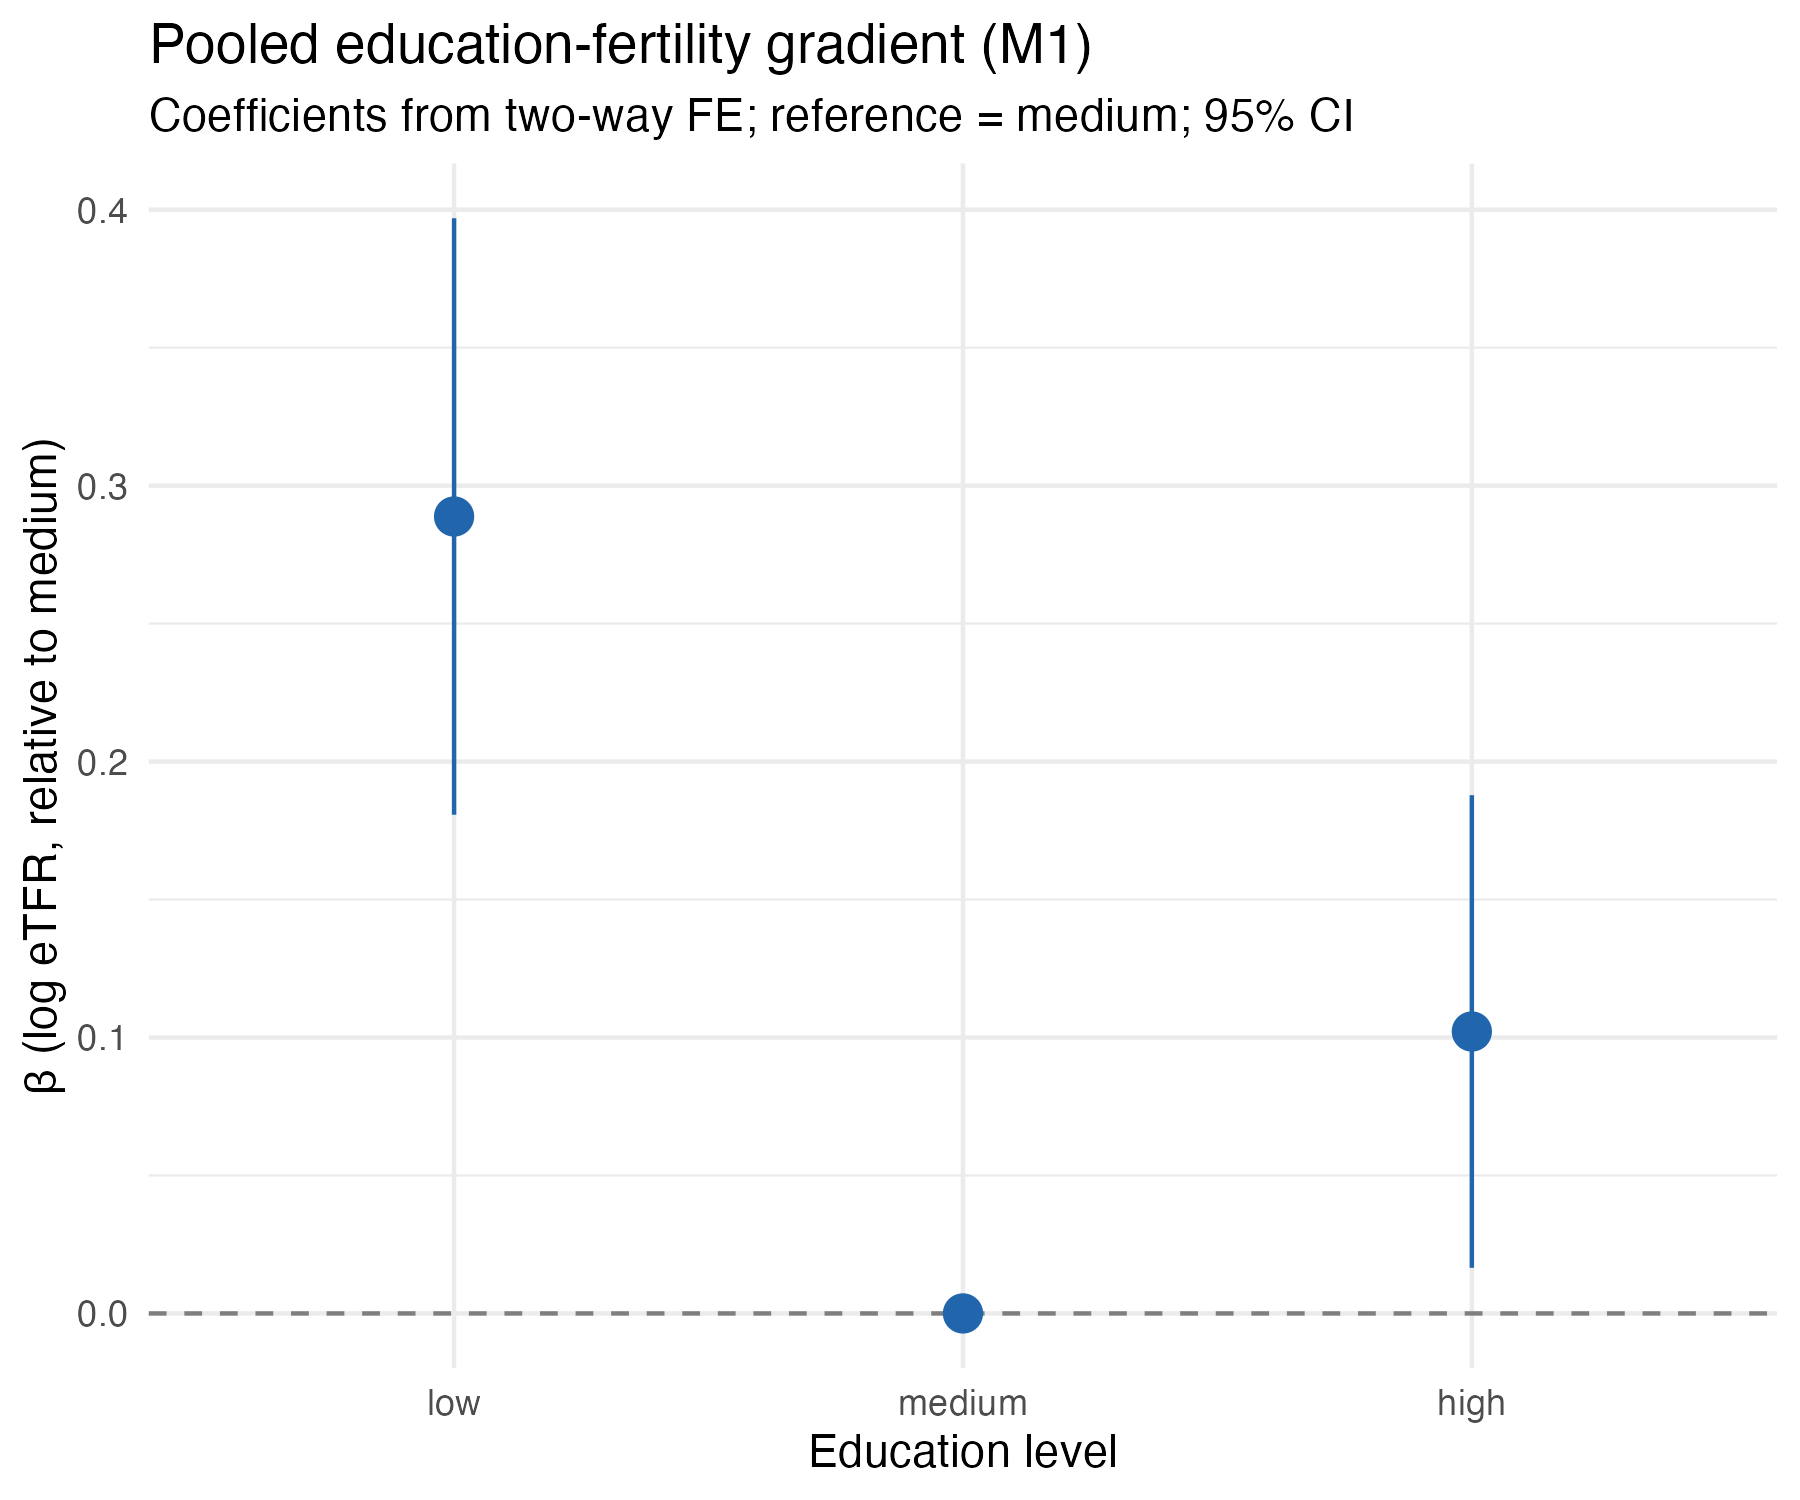
\includegraphics[width=0.8\textwidth]{h1_pooled_fe_coefs.png}
\caption{Pooled education--fertility gradient coefficients (M1), with 95\% confidence intervals from country-clustered standard errors. Reference: medium education.}
\label{fig:m1}
\end{figure}

\section{Cross-country heterogeneity}
The pooled estimates conceal heterogeneity. Introducing country $\times$ education interactions (M2,
Sweden as reference) raises the within $R^2$ from 0.294 to 0.593: country-specific deviations
account for an additional 30 percentage points of within-variation, so heterogeneity is
substantively important, not a nuisance. High-education interactions are absorbed by collinearity
with the fixed effects, but the identified medium and low interactions characterise each country's
divergence from the Swedish baseline. Table~\ref{tab:m2} reports selected examples, spanning
Slovakia's steep positive gradient, Spain's elevated monotonic one, Romania's pronounced V-shape, and
Denmark's inverted gradient. The variation documented here is precisely what the H3 analysis in
Chapter~6 attempts to explain.

\begin{table}[ht]
\centering
\caption{Selected country $\times$ education interactions from M2 (reference country: Sweden; education reference: high, absorbed by country fixed effects; within $R^2=0.593$).}
\label{tab:m2}
\small
\begin{tabular}{@{}lccl@{}}
\toprule
Country & Medium interaction & Low interaction & Interpretation \\
\midrule
Slovakia & $-0.236$ & $+0.430$ & Steepest positive gradient \\
Spain    & $+0.343$ & $+0.368$ & Strong monotonic negative \\
Latvia   & $-0.159$ & $+0.176$ & Compositional U-shape \\
Greece   & $-0.103$ & $+0.170$ & Broad U-shape \\
Romania  & $-0.577$ & $-0.203$ & Pronounced V-shape \\
Denmark  & $-0.255$ & $-0.510$ & Inverted gradient \\
T\"urkiye & $+0.152$ & $+0.177$ & Strong monotonic negative \\
\bottomrule
\end{tabular}
\end{table}

\section{Robustness checks on H1}
Table~\ref{tab:robust} reports M1 across four sensitivity checks alongside the baseline. The low--medium
coefficient is remarkably stable, ranging from $+0.244$ (excluding U-shape composition countries) to
$+0.379$ (balanced subsample) and distinguishable from zero in every case: the strict H1 finding is
robust to all four sensitivities. The high--medium coefficient is more sensitive. It remains positive
and significant in the baseline, balanced, and no-COVID specifications, but falls to $+0.089$
($p=0.216$) once the eight composition countries are removed, and to $+0.012$ ($p=0.890$), no longer
distinguishable from zero, under population weighting. The substantive implication is that the strict
negative gradient (low~$>$~high) is robust, but the U-shape's right arm visible in M1 is partly a
property of smaller countries with potentially composition-influenced low tiers and is not detectable
in a population-weighted analysis.
The U-shape is a feature of European countries as units more than of European women as a population, a
qualification carried forward honestly rather than suppressed.

\begin{table}[ht]
\centering
\caption{H1 robustness, M1 coefficients across four sensitivity specifications (two-way fixed effects, country-clustered SEs, reference: medium).}
\label{tab:robust}
\small
\begin{tabular}{@{}lccccc@{}}
\toprule
Specification & $N$ & Low $\beta$ (SE) & High $\beta$ (SE) & Low $p$ & High $p$ \\
\midrule
Baseline (M1)            & 933 & $+0.289$ (0.052) & $+0.102$ (0.041) & $<0.001$ & 0.022 \\
Balanced (8 countries)   & 432 & $+0.379$ (0.078) & $+0.143$ (0.059) & 0.002 & 0.045 \\
Excluding 2020--2021     & 840 & $+0.278$ (0.051) & $+0.097$ (0.042) & $<0.001$ & 0.033 \\
Excluding U-shape comp.  & 561 & $+0.244$ (0.059) & $+0.089$ (0.069) & 0.002 & 0.216 \\
Population-weighted       & 933 & $+0.253$ (0.044) & $+0.012$ (0.083) & $<0.001$ & 0.890 \\
\bottomrule
\end{tabular}
\end{table}

\subsection{Small-cluster inference: CR2 with Satterthwaite degrees of freedom}
\label{sec:cr2}
Table~\ref{tab:cr2} re-estimates the battery using the CR2 bias-reduced estimator with Satterthwaite
degrees of freedom \citep{pustejovskytipton2018}. The models are refitted with \texttt{lm} and country
and year entered as dummies, the same regression by the Frisch--Waugh--Lovell theorem; coefficients
agree with the fixed-effects estimates to numerical tolerance.

The correction makes no material difference. The CR2 standard errors are marginally \emph{smaller}
than the reported cluster-robust ones (ratios of 0.99), because \texttt{fixest} already applies a
finite-sample adjustment fractionally more conservative than CR2's bias reduction: the
uncorrected sandwich estimator gives 0.050 and 0.040 for the low and high contrasts, CR2 gives
0.051 and 0.041, and \texttt{fixest} gives 0.052 and 0.041. The Satterthwaite degrees of freedom
pull the other way (18.7 rather than 20 in the baseline), and the two effects offset.
The strict H1 contrast is $-0.187$ with $p=0.0015$ under both methods, and no coefficient changes
significance in any specification. The degrees of freedom behave as theory predicts, which checks the
implementation: the balanced subsample returns exactly $G-1=7$, the value Satterthwaite converges on
when clusters are balanced, while unbalanced specifications return values strictly below $G-1$. The
small-cluster concern raised in Section~3.5 is therefore empirically inert here, and the unavailability
of the wild-cluster bootstrap is not a material limitation for these data.

\begin{table}[ht]
\centering
\caption{H1 robustness under CR2 with Satterthwaite degrees of freedom (reference: medium). The population-weighted specification is omitted; weighted least squares requires separate treatment in \texttt{clubSandwich}.}
\label{tab:cr2}
\small
\begin{tabular}{@{}lccccccc@{}}
\toprule
Specification & $N$ & $G$ & Low $\beta$ (CR2 SE) & Low $p$ & High $\beta$ (CR2 SE) & High $p$ & df \\
\midrule
Baseline                 & 933 & 21 & $+0.289$ (0.051) & $<0.001$ & $+0.102$ (0.041) & 0.021 & 18.7 \\
Balanced (8 countries)   & 432 & 8  & $+0.379$ (0.076) & 0.002    & $+0.143$ (0.057) & 0.041 & 7.0 \\
Excluding 2020--2021     & 840 & 21 & $+0.278$ (0.051) & $<0.001$ & $+0.097$ (0.042) & 0.033 & 18.8 \\
Excluding U-shape comp.  & 561 & 13 & $+0.244$ (0.059) & 0.002    & $+0.089$ (0.068) & 0.212 & 11.1 \\
\bottomrule
\end{tabular}
\end{table}

\section{H2: quadratic specification}
H2 is tested first by adding a quadratic term in ordinally coded education
(Table~\ref{tab:quad}). The linear specification gives $\beta=-0.093$ ($p=0.002$), the conventional
H1 finding on the ordinal scale, but with a within $R^2$ of only 0.119, less than half that of M1,
the first sign that linearity is too restrictive. The quadratic specification produces a large
negative linear term ($\beta_1=-0.484$, $p<0.001$) and a positive quadratic term ($\beta_2=+0.195$,
$p<0.001$), raising the within $R^2$ to 0.294. The Wald test on $\beta_2=0$ gives $F(1,20)=24.8$
($p=7.16\times10^{-5}$). Note that with three education levels and two parameters (plus fixed
effects), the quadratic specification saturates the education dimension, its within $R^2$ of 0.294
matches M1's categorical specification by construction, and the $\Delta\mathrm{AIC}=-204$ against the
linear form reflects the gain from a constrained to a saturated model, not independent evidence for
curvature. The quadratic is nonetheless a convenient summary that locates the minimum at education
$=1.24$ on the ordinal scale, between the medium and high tiers, closer to medium, consistent with
the descriptive ordering, and the positive $\beta_2$ directly parameterises the U-shape established
by M1's two positive coefficients. Translated back to the fertility scale, predicted relative eTFR is 1.00 at low, 0.75 at
medium, and 0.83 at high: medium-educated women are predicted to have about 25\% lower fertility than
low-educated women, with an 8-percentage-point recovery from medium to high (approximately
$+10.7\%$ in proportional terms), the parametric counterpart of the U-shape's right arm. H2 is therefore confirmed parametrically.

\begin{table}[ht]
\centering
\caption{H2, linear vs quadratic education specifications. Two-way fixed effects, country-clustered SEs, $N=933$.}
\label{tab:quad}
\begin{tabular}{@{}lcc@{}}
\toprule
Term / statistic & Linear & Quadratic \\
\midrule
educ ($\beta_1$)   & $-0.093$ (0.025), $p=0.002$ & $-0.484$ (0.088), $p<0.001$ \\
educ$^2$ ($\beta_2$) & -- & $+0.195$ (0.039), $p<0.001$ \\
Within $R^2$ & 0.119 & 0.294 \\
AIC & $-213.0$ & $-417.0$ \\
BIC & $-24.3$ & $-223.5$ \\
Curve minimum (educ) & -- & 1.24 \\
\bottomrule
\end{tabular}
\end{table}

\begin{figure}[ht]
\centering
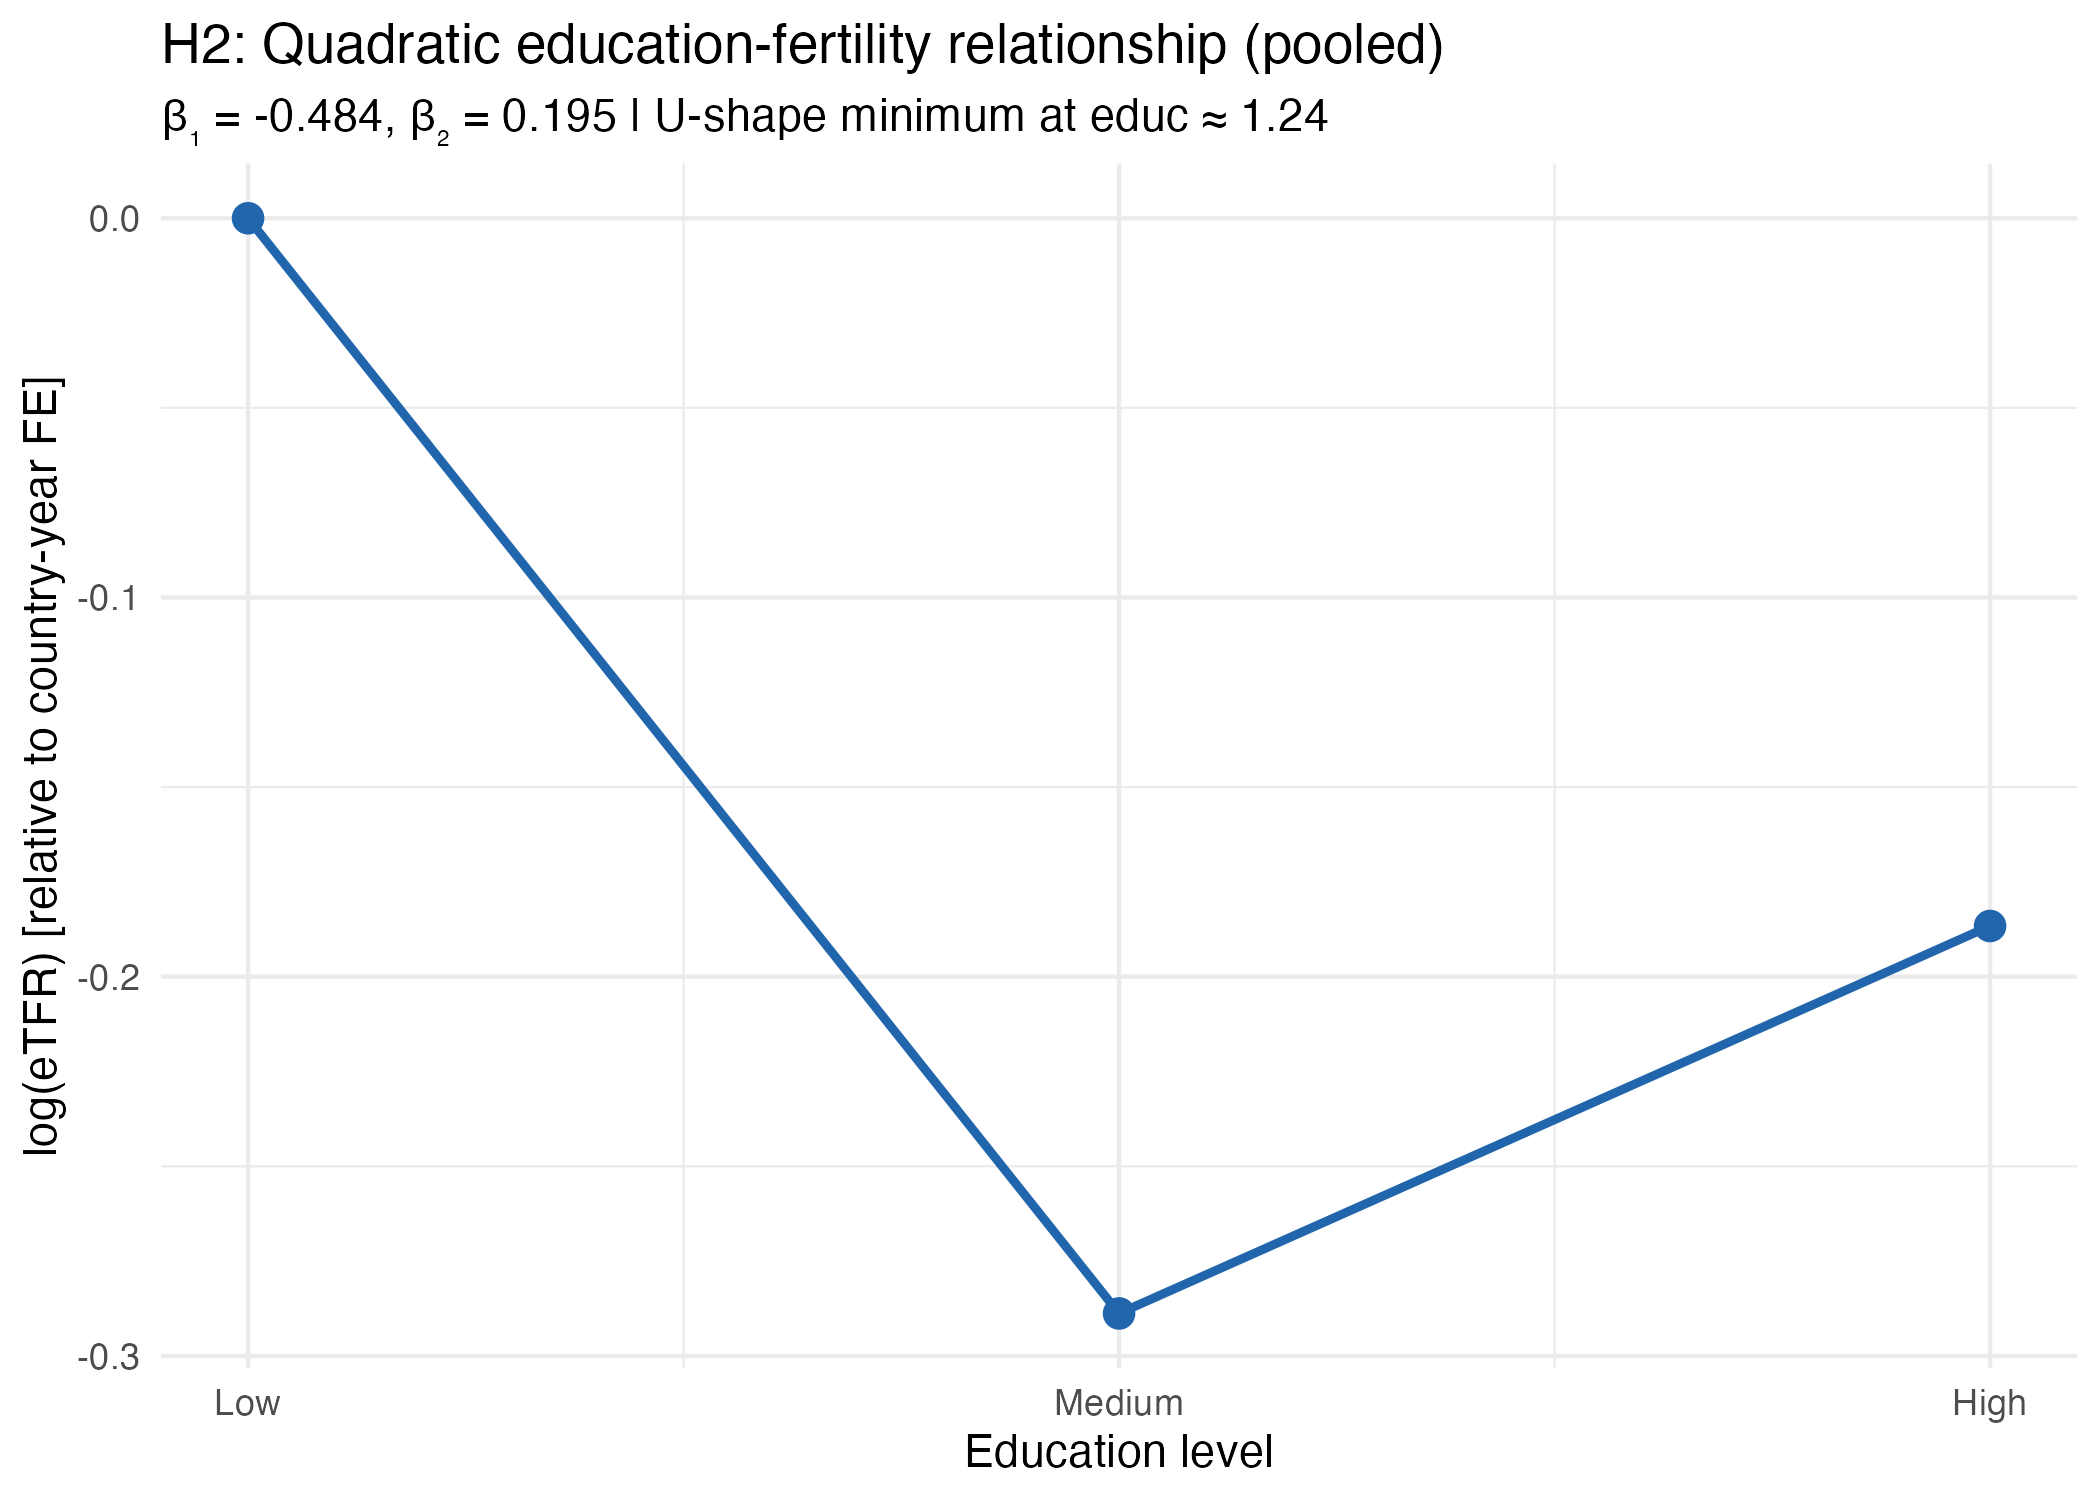
\includegraphics[width=0.8\textwidth]{h2_quadratic_curve.png}
\caption{Predicted log eTFR from the quadratic specification, relative to the country--year fixed-effects baseline. The curve attains its minimum at educ $\approx 1.24$. $\beta_1=-0.484$, $\beta_2=+0.195$.}
\label{fig:quad}
\end{figure}

\section{H2: quantile regression across the distribution}
Quantile regression at $\tau\in\{0.10,0.25,0.50,0.75,0.90\}$ (reference: high) tests whether the
U-shape is stable across the conditional distribution (Table~\ref{tab:quant}). Standard errors come
from a bootstrap clustered by country ($R=1{,}000$, weighted \textit{xy} method), implemented
through the \texttt{quantreg} package's bootstrap facility. Clustering matters substantially here: the clustered
standard errors are 2.5 to 3.1 times larger than their unclustered counterparts across all five
quantiles, so an unclustered bootstrap would have overstated precision at every point in the
distribution.

The point estimates trace a U at every quantile: the low-versus-high coefficient is positive
throughout (from $+0.093$ to $+0.280$) and the medium-versus-high coefficient negative throughout
(from $-0.119$ to $-0.064$). Statistical identification, however, is confined to the middle of the
distribution. The medium--high contrast is distinguishable from zero at $\tau=0.25$, $0.50$, and
$0.75$ but not at $\tau=0.10$ ($p=0.065$) or $\tau=0.90$ ($p=0.154$); the low--high contrast is
significant at every quantile except $\tau=0.10$ ($p=0.233$). This is imprecision rather than evidence
of absence, since quantile regression is least precise in the tails, but the honest reading is that the
U-shape is identified in the central portion of the distribution and merely suggested at its extremes.
Two nuances survive: the low--high gap widens as $\tau$ rises, so the conventional gradient is more
pronounced in high-fertility cells, while the medium--high gap narrows, so the U-shape's right arm
flattens at high fertility. The U-shape's sign is stable across the distribution; its strength and
statistical identification are not.

\begin{table}[ht]
\centering
\caption{H2, quantile regression coefficients for education contrasts (reference: high) at five quantiles of log eTFR, with country-clustered bootstrap standard errors in parentheses ($R=1{,}000$). $N=933$.}
\label{tab:quant}
\begin{tabular}{@{}lccccc@{}}
\toprule
Contrast (ref = high) & $\tau=0.10$ & $\tau=0.25$ & $\tau=0.50$ & $\tau=0.75$ & $\tau=0.90$ \\
\midrule
Low    & $+0.093$ & $+0.140$ & $+0.205$ & $+0.236$ & $+0.280$ \\
       & (0.078) & (0.061) & (0.053) & (0.059) & (0.062) \\
       & $p=0.233$ & $p=0.021$ & $p<0.001$ & $p<0.001$ & $p<0.001$ \\
\addlinespace
Medium & $-0.119$ & $-0.129$ & $-0.102$ & $-0.091$ & $-0.064$ \\
       & (0.065) & (0.048) & (0.036) & (0.042) & (0.045) \\
       & $p=0.065$ & $p=0.007$ & $p=0.005$ & $p=0.032$ & $p=0.154$ \\
\bottomrule
\end{tabular}
\end{table}

\begin{figure}[ht]
\centering
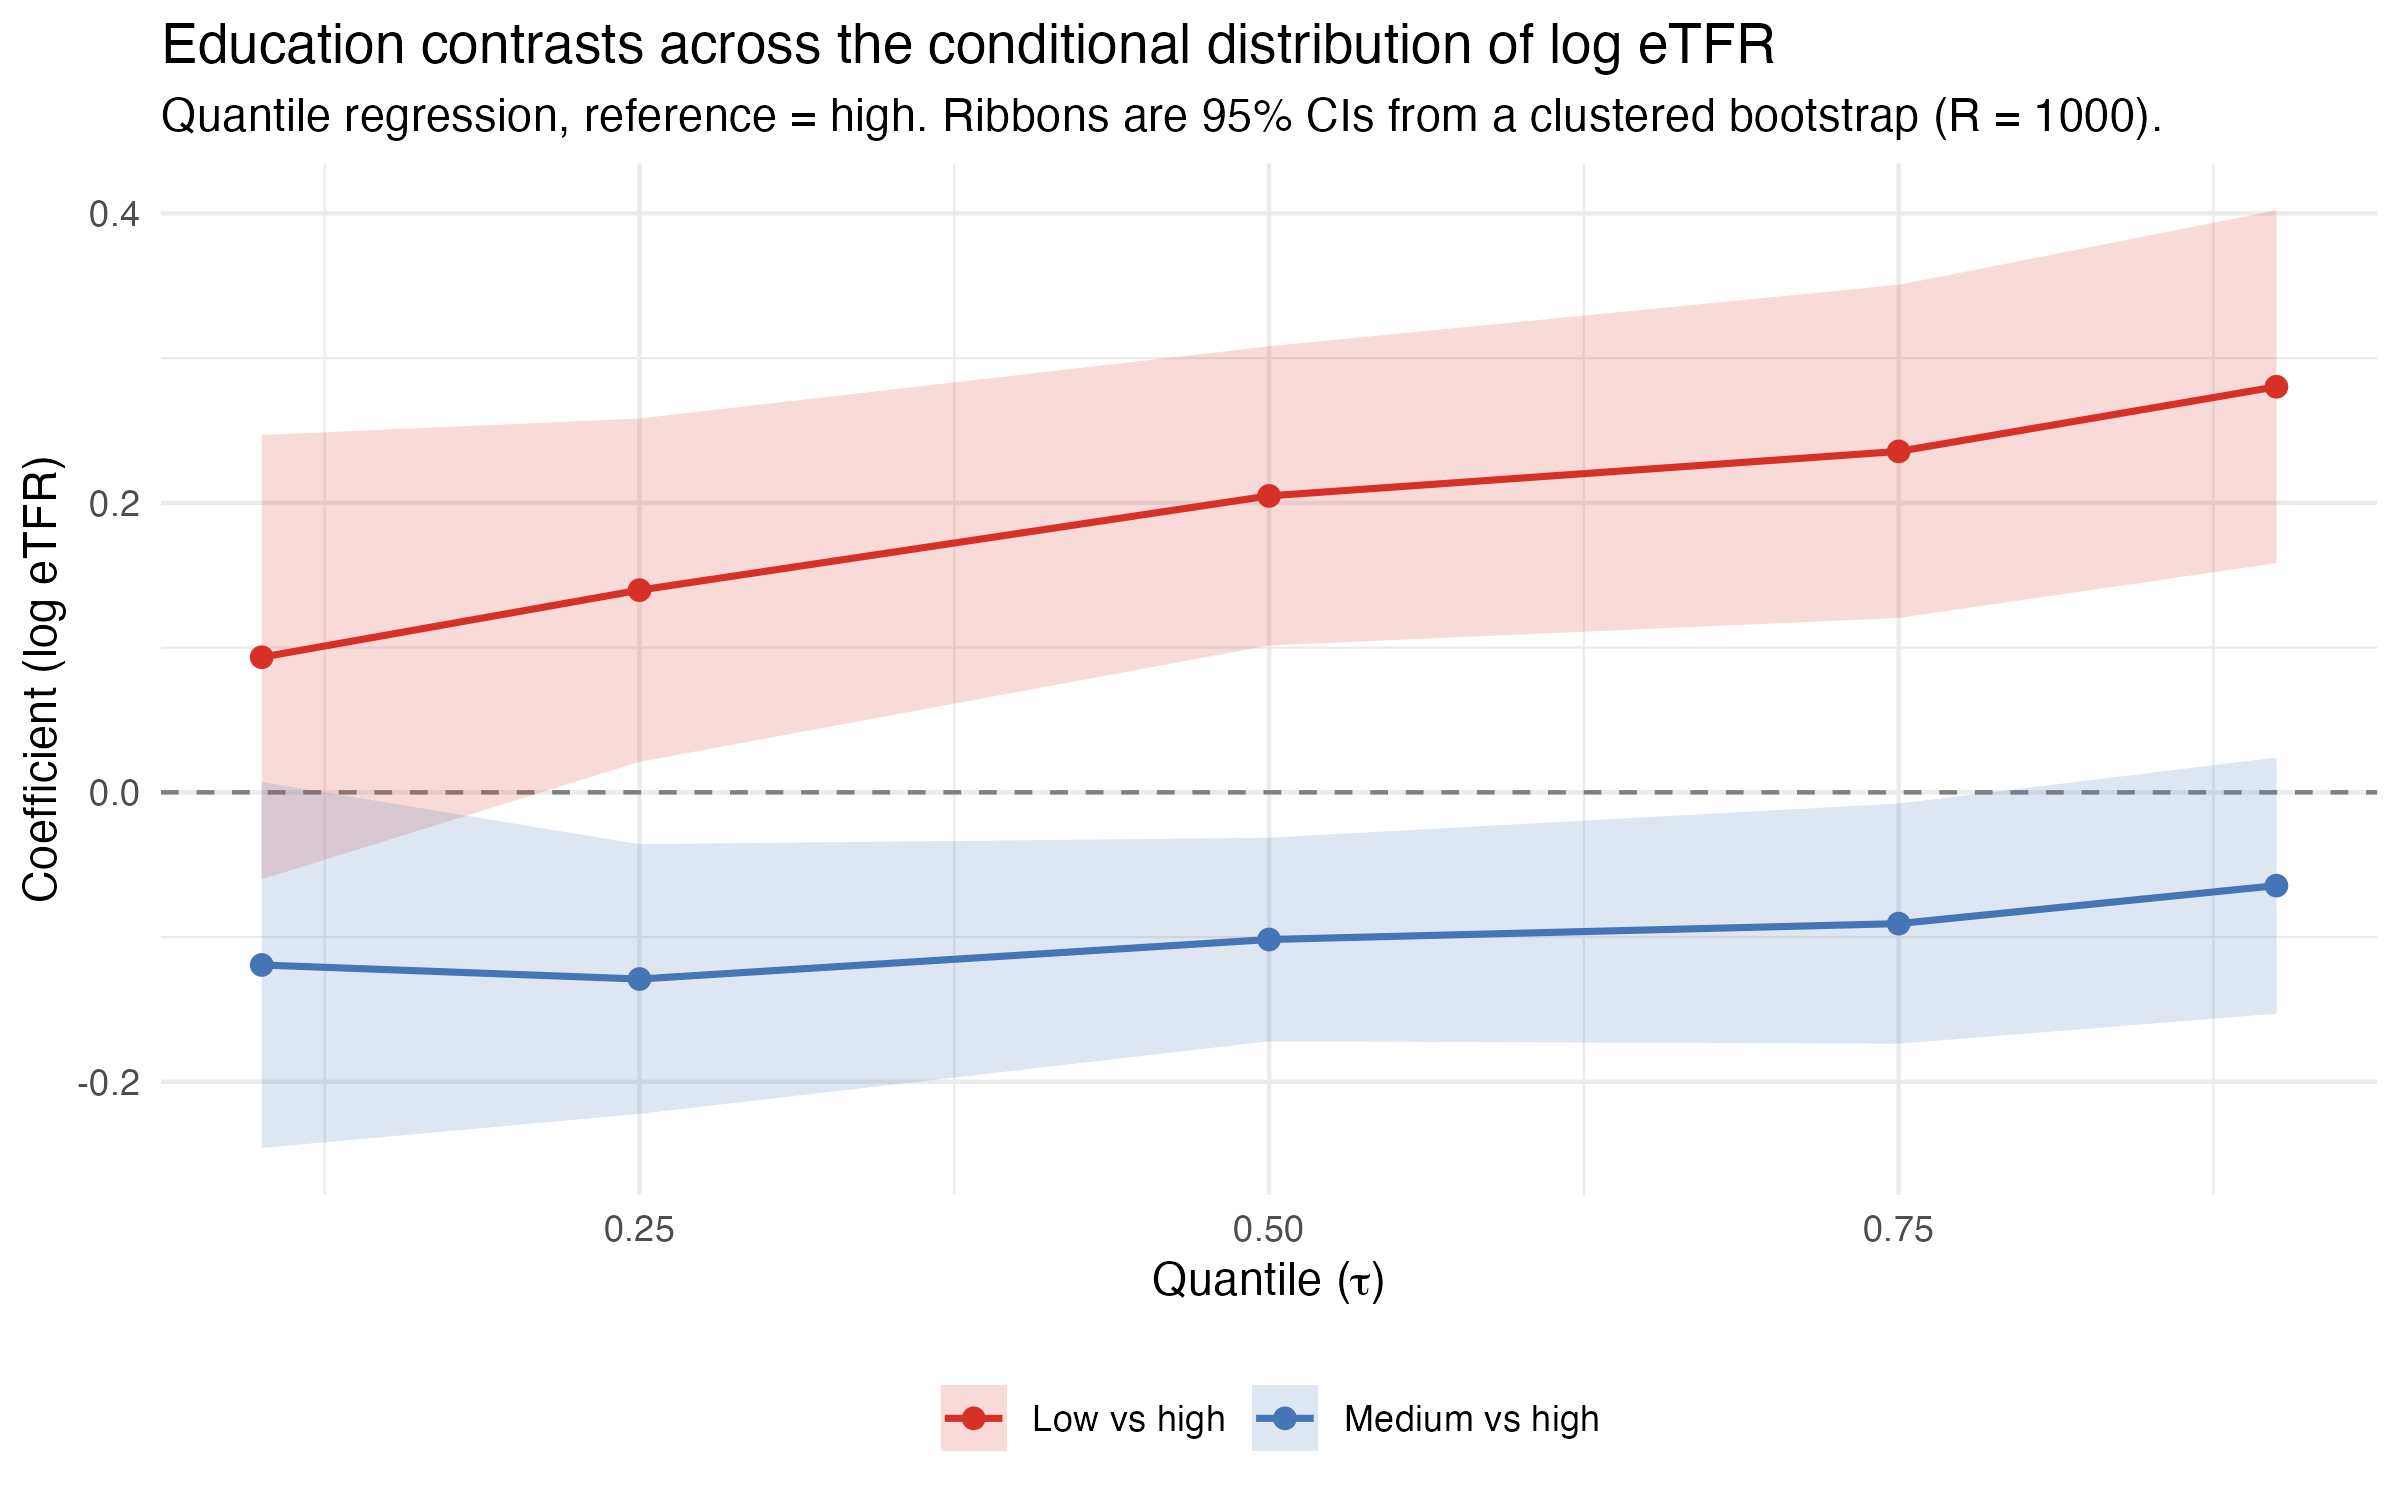
\includegraphics[width=0.8\textwidth]{h2_quantile_boot.png}
\caption{Education contrasts across the conditional distribution of log eTFR, from quantile regressions at five quantiles (reference: high). Ribbons are 95\% confidence intervals from a country-clustered bootstrap ($R=1{,}000$). The low--high gap rises across $\tau$; the medium--high gap narrows and its interval covers zero at $\tau=0.90$.}
\label{fig:quant}
\end{figure}

\section{Summary}
H1 is confirmed by the high--low contrast ($\beta=-0.187$, $p=0.002$) and is robust to the four
sensitivity checks in Table~\ref{tab:robust}. H2 is confirmed parametrically ($\beta_2=+0.195$,
$p<0.001$, with an interior minimum at educ~$=1.24$) and, in the central portion of the
distribution, distributionally. Three qualifications attach. First, the U-shape's medium-to-high
recovery is not robust to population
weighting, so it characterises European countries as units more than European women as a
population. Second, its statistical identification is confined to the middle of the
conditional distribution. Third, and most consequentially, the H1 result is
sensitive to the age range over which the eTFR is computed, developed in
Section~\ref{sec:agefloor}. The cross-country heterogeneity (M2 within $R^2=0.593$) motivates the
H3 analysis, and the turn to the individual level under H4, both in Chapter~6.

\section{The age range of the eTFR: timing versus quantum}
\label{sec:agefloor}
Section~\ref{sec:etfr} flagged that the uniform-attainment assumption is weakest at the youngest
ages, where education is still in progress. Because those cells feed the low tier, the gradient
could in principle be an artefact of them. Table~\ref{tab:agefloor} rebuilds the eTFR over
progressively narrower age ranges and re-runs the H1 and H2 tests on each.

\begin{table}[ht]
\centering
\caption{H1 and H2 across three age ranges of the eTFR. Two-way fixed effects, country-clustered SEs, $N=933$ throughout (the restriction changes the age groups summed, not the country--year--education cells).}
\label{tab:agefloor}
\small
\begin{tabular}{@{}lccccc@{}}
\toprule
eTFR age range & Low vs medium & High vs medium & High vs low (H1) & $\beta_2$ (H2) & Curve min. \\
\midrule
15--49 (baseline) & $+0.289^{***}$ & $+0.102^{*}$   & $-0.187^{**}$ & $+0.195^{***}$ & 1.24 \\
20--49            & $+0.317^{***}$ & $+0.160^{**}$  & $-0.157^{**}$ & $+0.238^{***}$ & 1.16 \\
25--49            & $+0.016$       & $+0.217^{***}$ & $+0.201^{**}$ & $+0.116^{*}$   & 0.57 \\
\bottomrule
\end{tabular}

\vspace{0.5em}
\footnotesize{$^{*}p<0.05$; $^{**}p<0.01$; $^{***}p<0.001$.}
\end{table}

The result is stark. Dropping ages 15--19 barely moves the H1 contrast ($-0.187$ to $-0.157$).
Dropping ages 20--24 reverses its sign ($+0.201$, $p=0.002$): among women aged 25 and over,
high-educated women have \emph{higher} period fertility than low-educated women. The
low--medium contrast collapses to zero ($+0.016$, $p=0.787$). The entire conventional negative
gradient is located in ages 20--24.

Two readings are available, and the composition of the age groups adjudicates between them. At
ages 15--19, 82\% of women are classified low-educated and almost none as high, because
upper secondary is not yet complete; the low tier there is a mechanical rather than a behavioural
category. Were the reversal driven by those cells it would be an artefact, but it is not: they
contribute only 3.2\% of the low tier's eTFR and a negligible 0.2\% of the high tier's. At ages
20--24, by contrast, 14.0\% of women are classified low-educated, almost exactly the 13.8\% observed
at 25--29, so the low tier there is not mechanically inflated; those women contribute 35.0\% of the low
tier's total eTFR against 9.9\% for the high tier.

The reversal is therefore substantive rather than artefactual, and it identifies the negative
gradient as a phenomenon of \emph{timing}. Low-educated women concentrate childbearing at 20--24;
high-educated women concentrate it at 30--34, which supplies 37.2\% of their eTFR. Period measures
conflate the tempo and quantum of fertility \citep{bongaartsfeeney1998,kohlerphilipov2001}, and
neither range identifies completed fertility by final attainment, which is the quantity the
paradox is properly about.

What survives the sweep is the U-shape. Medium-educated women record the lowest mean eTFR at every
age floor (1.36 against 1.85 and 1.51 at 15--49; 1.10 against 1.15 and 1.36 at 25--49), and
$\beta_2$ remains positive with an interior minimum throughout. The qualification is that which
\emph{arm} of the U is statistically identified depends on the specification: the left arm
(low above medium) is not identified at 25--49, and the right arm (high above medium) is not
identified under population weighting. Only in the full panel are both arms significant. The
non-monotonicity is thus the more robust of the two findings, and the conventional negative gradient
the more fragile, the reverse of the ordering the literature assumes.

% ==========================================================================
% CHAPTER 6
% ==========================================================================
\chapter{Mechanism Results: H3 and H4}

This chapter turns to mechanism. H3 asks whether cross-country variation in the gradient is better
predicted by cultural than by economic indicators; H4 asks whether the individual education effect is
mediated primarily by attitudinal rather than economic pathways. Both concern whether cultural or
economic processes dominate the contemporary relationship, at different levels of analysis.

\section{H3 Stage 1: XGBoost discovery and SHAP decomposition}
The gradient-boosted regression of country-level gradient steepness on all twelve predictors selected
13 boosting rounds by cross-validation. Out-of-sample performance is poor: the LOOCV $R^2$ is
$-0.086$, meaning the fitted model predicts the held-out country slightly worse than the training
mean. At $N=21$ the macro indicators carry no reliable out-of-sample predictive power, a substantive
finding in its own right, so I use the SHAP decomposition (Table~\ref{tab:shap}) only to identify
in-sample signal, reserving inference for Stage~2. Three predictors dominate: freedom of religion
(institutional, 44.9\%), contraceptive prevalence (22.2\%), and GDP per capita (18.3\%), together
85.4\% of the signal; five predictors receive zero importance under the regularisation. Aggregated by
category, attitudinal predictors account for 5.4\%, institutional for 54.1\%, and economic for 40.5\%.
Combining the institutional and attitudinal shares into a non-economic block (59.5\%), with the caveat
from Section~3.3 that the V-Dem indices measure institutional structure rather than individual
attitudes, that block exceeds the economic one. Two features qualify this. Contraceptive
prevalence is classified as economic because it proxies access to modern fertility
control, but could be assigned to the cultural block as a proximate
determinant reflecting normative conditions; reclassifying it shifts the cultural share to 81.7\%, so
the comparison is sensitive to one coding decision. It is also the predictor with the weakest coverage,
observed for only 12 of 21 countries, so 22.2\% of in-sample importance rests on data
present for 57\% of the panel. Read at face value the block comparison favours H3, but the cultural share is
almost entirely carried by a single institutional predictor (freedom of religion); strip it out, and the blocks are roughly equal. This
dependence on one feature, together with the negative LOOCV $R^2$, motivates the parsimonious Stage~2.

\begin{table}[ht]
\centering
\caption{H3 Stage 1, SHAP feature importance (mean $|\mathrm{SHAP}|$, in-sample fit; LOOCV $R^2=-0.086$).}
\label{tab:shap}
\small
\begin{tabular}{@{}lccc@{}}
\toprule
Feature & Mean $|\mathrm{SHAP}|$ & Group & Share \\
\midrule
relig\_free   & 0.0263 & Institutional & 44.9\% \\
contraceptive & 0.0130 & Economic & 22.2\% \\
gdp\_percap   & 0.0107 & Economic & 18.3\% \\
polyarchy     & 0.0031 & Institutional & 5.3\% \\
libdem        & 0.0023 & Institutional & 3.9\% \\
ess\_secular  & 0.0022 & Attitudinal & 3.8\% \\
ess\_autonomy & 0.0009 & Attitudinal & 1.6\% \\
gender\_equal, egaldem, flfp, ess\_gender\_egal, post\_socialist & 0.0000 & Mixed & 0.0\% \\
\bottomrule
\end{tabular}
\end{table}

\begin{figure}[ht]
\centering
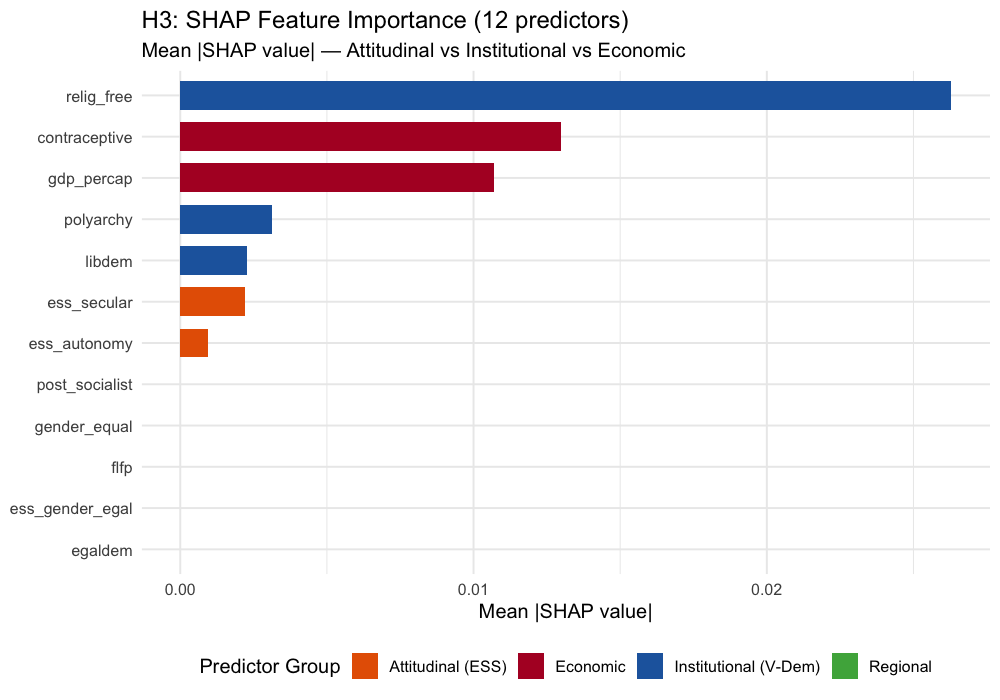
\includegraphics[width=0.8\textwidth]{h3_shap_importance.png}
\caption{H3 Stage 1, mean absolute SHAP values across the twelve predictors, coloured by theoretical category. Seven of twelve are non-zero; five are absorbed by regularisation.}
\label{fig:shapimp}
\end{figure}

\begin{figure}[ht]
\centering

\includegraphics[width=0.8\textwidth]{h3_shap_beeswarm.png}
\caption{H3 Stage 1, SHAP value distribution by country. Each dot is one country; positive values push predicted gradient steepness upward.}
\label{fig:shapbee}
\end{figure}

\section{H3 Stage 2: Bayesian model comparison}
Six Bayesian models on the complete-case $N=18$ converged cleanly (maximum $\hat{R}=1.003$).
Table~\ref{tab:waic} reports the WAIC comparison: the economic model (GDP per capita plus female
labour-force participation) is best on both WAIC and LOO, with institutional and attitudinal models
close behind and combined specifications worst. Two observations qualify the ranking. The economic model is not distinguishable from the
institutional, attitudinal or updated-combined specifications, whose $\Delta\mathrm{ELPD}$ values lie
within two standard errors of zero, but it does outperform the post-socialist and
original-combined models by more than two standard errors. Within the cultural block the ESS
attitudinal model (M5)
outperforms the V-Dem institutional model (M1) by $\Delta\mathrm{ELPD}=+0.5$, reversing the
SHAP-based finding that institutional indicators dominate. Posterior summaries (Table~\ref{tab:post})
show GDP per capita the most precisely identified single predictor across all six models (median
$-0.27$, $P(<0)=0.97$): richer countries have flatter gradients. The ESS gender-egalitarianism
coefficient is negative (median $-0.15$, $P(<0)=0.91$), indicating that more gender-egalitarian
countries have flatter conventional gradients, consistent with the descriptive
finding that the Nordics display flatter or inverted gradients. Freedom of religion, the Stage~1
leader, has a posterior median of only $-0.12$ ($P(<0)=0.85$), far weaker than its SHAP rank implied.
Every credible interval crosses zero.

\begin{table}[ht]
\centering
\caption{H3 Stage 2, Bayesian model comparison by WAIC ($N=18$). The economic model is WAIC-best; LOO gives an identical ordering.}
\label{tab:waic}
\small
\begin{tabular}{@{}llcc@{}}
\toprule
Model & Specification & $\Delta\mathrm{ELPD}$ (WAIC) & SE \\
\midrule
M2 Economic         & gdp\_percap + flfp & 0.0 & -- \\
M3 Post-socialist   & post\_socialist & $-1.1$ & 0.5 \\
M5 Attitudinal      & ess\_secular + ess\_gender\_egal & $-1.4$ & 1.1 \\
M1 Institutional    & gender\_equal + relig\_free & $-1.9$ & 1.0 \\
M6 Updated combined & ess\_secular + gdp\_percap + post\_socialist & $-2.1$ & 1.2 \\
M4 Combined (orig.) & gender\_equal + flfp + post\_socialist & $-3.1$ & 0.6 \\
\bottomrule
\end{tabular}
\end{table}

\begin{table}[ht]
\centering
\caption{H3 Stage 2, posterior summaries for selected parameters (standardised predictors; common $N=18$).}
\label{tab:post}
\small
\begin{tabular}{@{}lcccc@{}}
\toprule
Parameter (model) & Median & SD & 95\% CrI & $P(\text{direction})$ \\
\midrule
gdp\_percap (M2)      & $-0.27$ & 0.15 & $[-0.57,\,+0.02]$ & $P(<0)=0.966$ \\
flfp (M2)             & $+0.16$ & 0.15 & $[-0.13,\,+0.46]$ & $P(>0)=0.873$ \\
ess\_gender\_egal (M5) & $-0.15$ & 0.12 & $[-0.38,\,+0.08]$ & $P(<0)=0.910$ \\
ess\_secular (M5)     & $+0.04$ & 0.12 & $[-0.19,\,+0.27]$ & $P(>0)=0.648$ \\
relig\_free (M1)      & $-0.12$ & 0.12 & $[-0.35,\,+0.12]$ & $P(<0)=0.853$ \\
gender\_equal (M1)    & $+0.01$ & 0.12 & $[-0.23,\,+0.25]$ & $P(>0)=0.531$ \\
\bottomrule
\end{tabular}
\end{table}

\begin{figure}[ht]
\centering

\includegraphics[width=0.8\textwidth]{h3_bayesian_posteriors.png}
\caption{H3 Stage 2, posterior distributions for the institutional (M1), attitudinal (M5), and economic (M2) models. Points and intervals are posterior medians and 95\% credible intervals; all intervals cross zero.}
\label{fig:post}
\end{figure}

\section{H3 synthesis}
Stage~1 ranks the cultural block at 59.5\% of in-sample importance; Stage~2 ranks the economic model
best on WAIC and LOO. Rather than suppressing this disagreement I treat it as the principal H3
finding: the discovery--inference design was built to surface exactly such divergences. The LOOCV
$R^2$ of $-0.086$ shows that the in-sample importance does not generalise, while GDP per capita
carries a posterior signal sufficient to make the economic model the most predictively reliable. No
model produces a definitive ranking at this sample size, the economic block holding a narrow edge on
Stage~2 criteria, the institutional block on Stage~1 SHAP, and all credible intervals crossing zero, so
the cross-country heterogeneity of Chapter~5 cannot be attributed to any single family of macro
indicators at $N=21$. Tellingly, the post-socialist dummy alone ($\Delta\mathrm{ELPD}=-1.1$)
outperforms both the attitudinal ($-1.4$) and institutional ($-1.9$) models: unmodelled regional
heterogeneity captures as much variation as any theoretically motivated predictor set. One nuance
survives: within the cultural block the attitudinal model edges the institutional one
($\Delta\mathrm{ELPD}=+0.5$), though the difference is well within both models' standard errors. The
direction is consistent with the cultural-evolutionary account in which the relevant unit is the
individual mind rather than formal institutional architecture.

A limitation of the outcome compounds these constraints. Gradient steepness is
defined over ages 15--49, and Section~\ref{sec:agefloor} shows that this quantity is located almost
entirely in ages 20--24 and reverses when cumulated over ages 25--49. The H3 outcome therefore inherits
the tempo character of the H1 contrast: what the country-level models explain is cross-national
variation in how far low-educated women concentrate childbearing in their early twenties, not variation
in a completed-fertility differential. This is a further reason to read the H3 results as
provisional and to prefer the U-shape indicator, stable at every age floor tested, as the more robust
characterisation of gradient shape. Recomputing steepness on a 25--49 basis and refitting the six
models is the first extension the design invites.

\section{H4: total causal effect of education on completed fertility}
The DML total effect (Table~\ref{tab:dml}) is estimated under a partially linear model with ten
pre-treatment confounders. Figure~\ref{fig:rawgrad} shows the unadjusted gradient: women's fertility
falls steeply with qualifications (2.12 children at the lowest tier to 1.57 at NVQ4+), men's more
modestly. Notably, women's fertility is flat across the top two tiers, 1.57 at both NVQ3 and NVQ4+, echoing
the macro-level H2 finding that the gradient flattens or recovers at the
top of the education distribution. For women, one additional NVQ level reduces completed fertility by 0.133 children
($p<0.001$, $N=1{,}461$), about 0.53 fewer children across the full NVQ range, surviving extensive
adjustment for cognitive ability and family background, so the effect is not attributable to selection
on observed pre-treatment characteristics. The sample drops from the 4,445 women with non-missing
outcome, treatment, and sex to 1,461 because complete cases on all ten
pre-treatment confounders are required; this reduction occurs before any mediator enters.
For men the effect is smaller ($-0.047$) and not
distinguishable from zero ($p=0.148$), consistent with the literature in which education's fertility
effect operates primarily through women \citep{skirbekk2008}. The mediation analysis is therefore
interpreted principally for women.

\begin{table}[ht]
\centering
\caption{H4, total causal effect of education on completed fertility (DML partially linear regression); $\theta$ is the effect of one additional NVQ level.}
\label{tab:dml}
\begin{tabular}{@{}lcccc@{}}
\toprule
Sample & $N$ & $\theta$ (SE) & 95\% CI & $p$ \\
\midrule
Women  & 1{,}461 & $-0.133$ (0.028) & $[-0.188,\,-0.078]$ & $<0.001$ \\
Men    & 1{,}081 & $-0.047$ (0.033) & $[-0.112,\,+0.017]$ & 0.148 \\
Pooled & 2{,}542 & $-0.110$ (0.022) & $[-0.153,\,-0.067]$ & $<0.001$ \\
\bottomrule
\end{tabular}
\end{table}

\begin{figure}[ht]
\centering
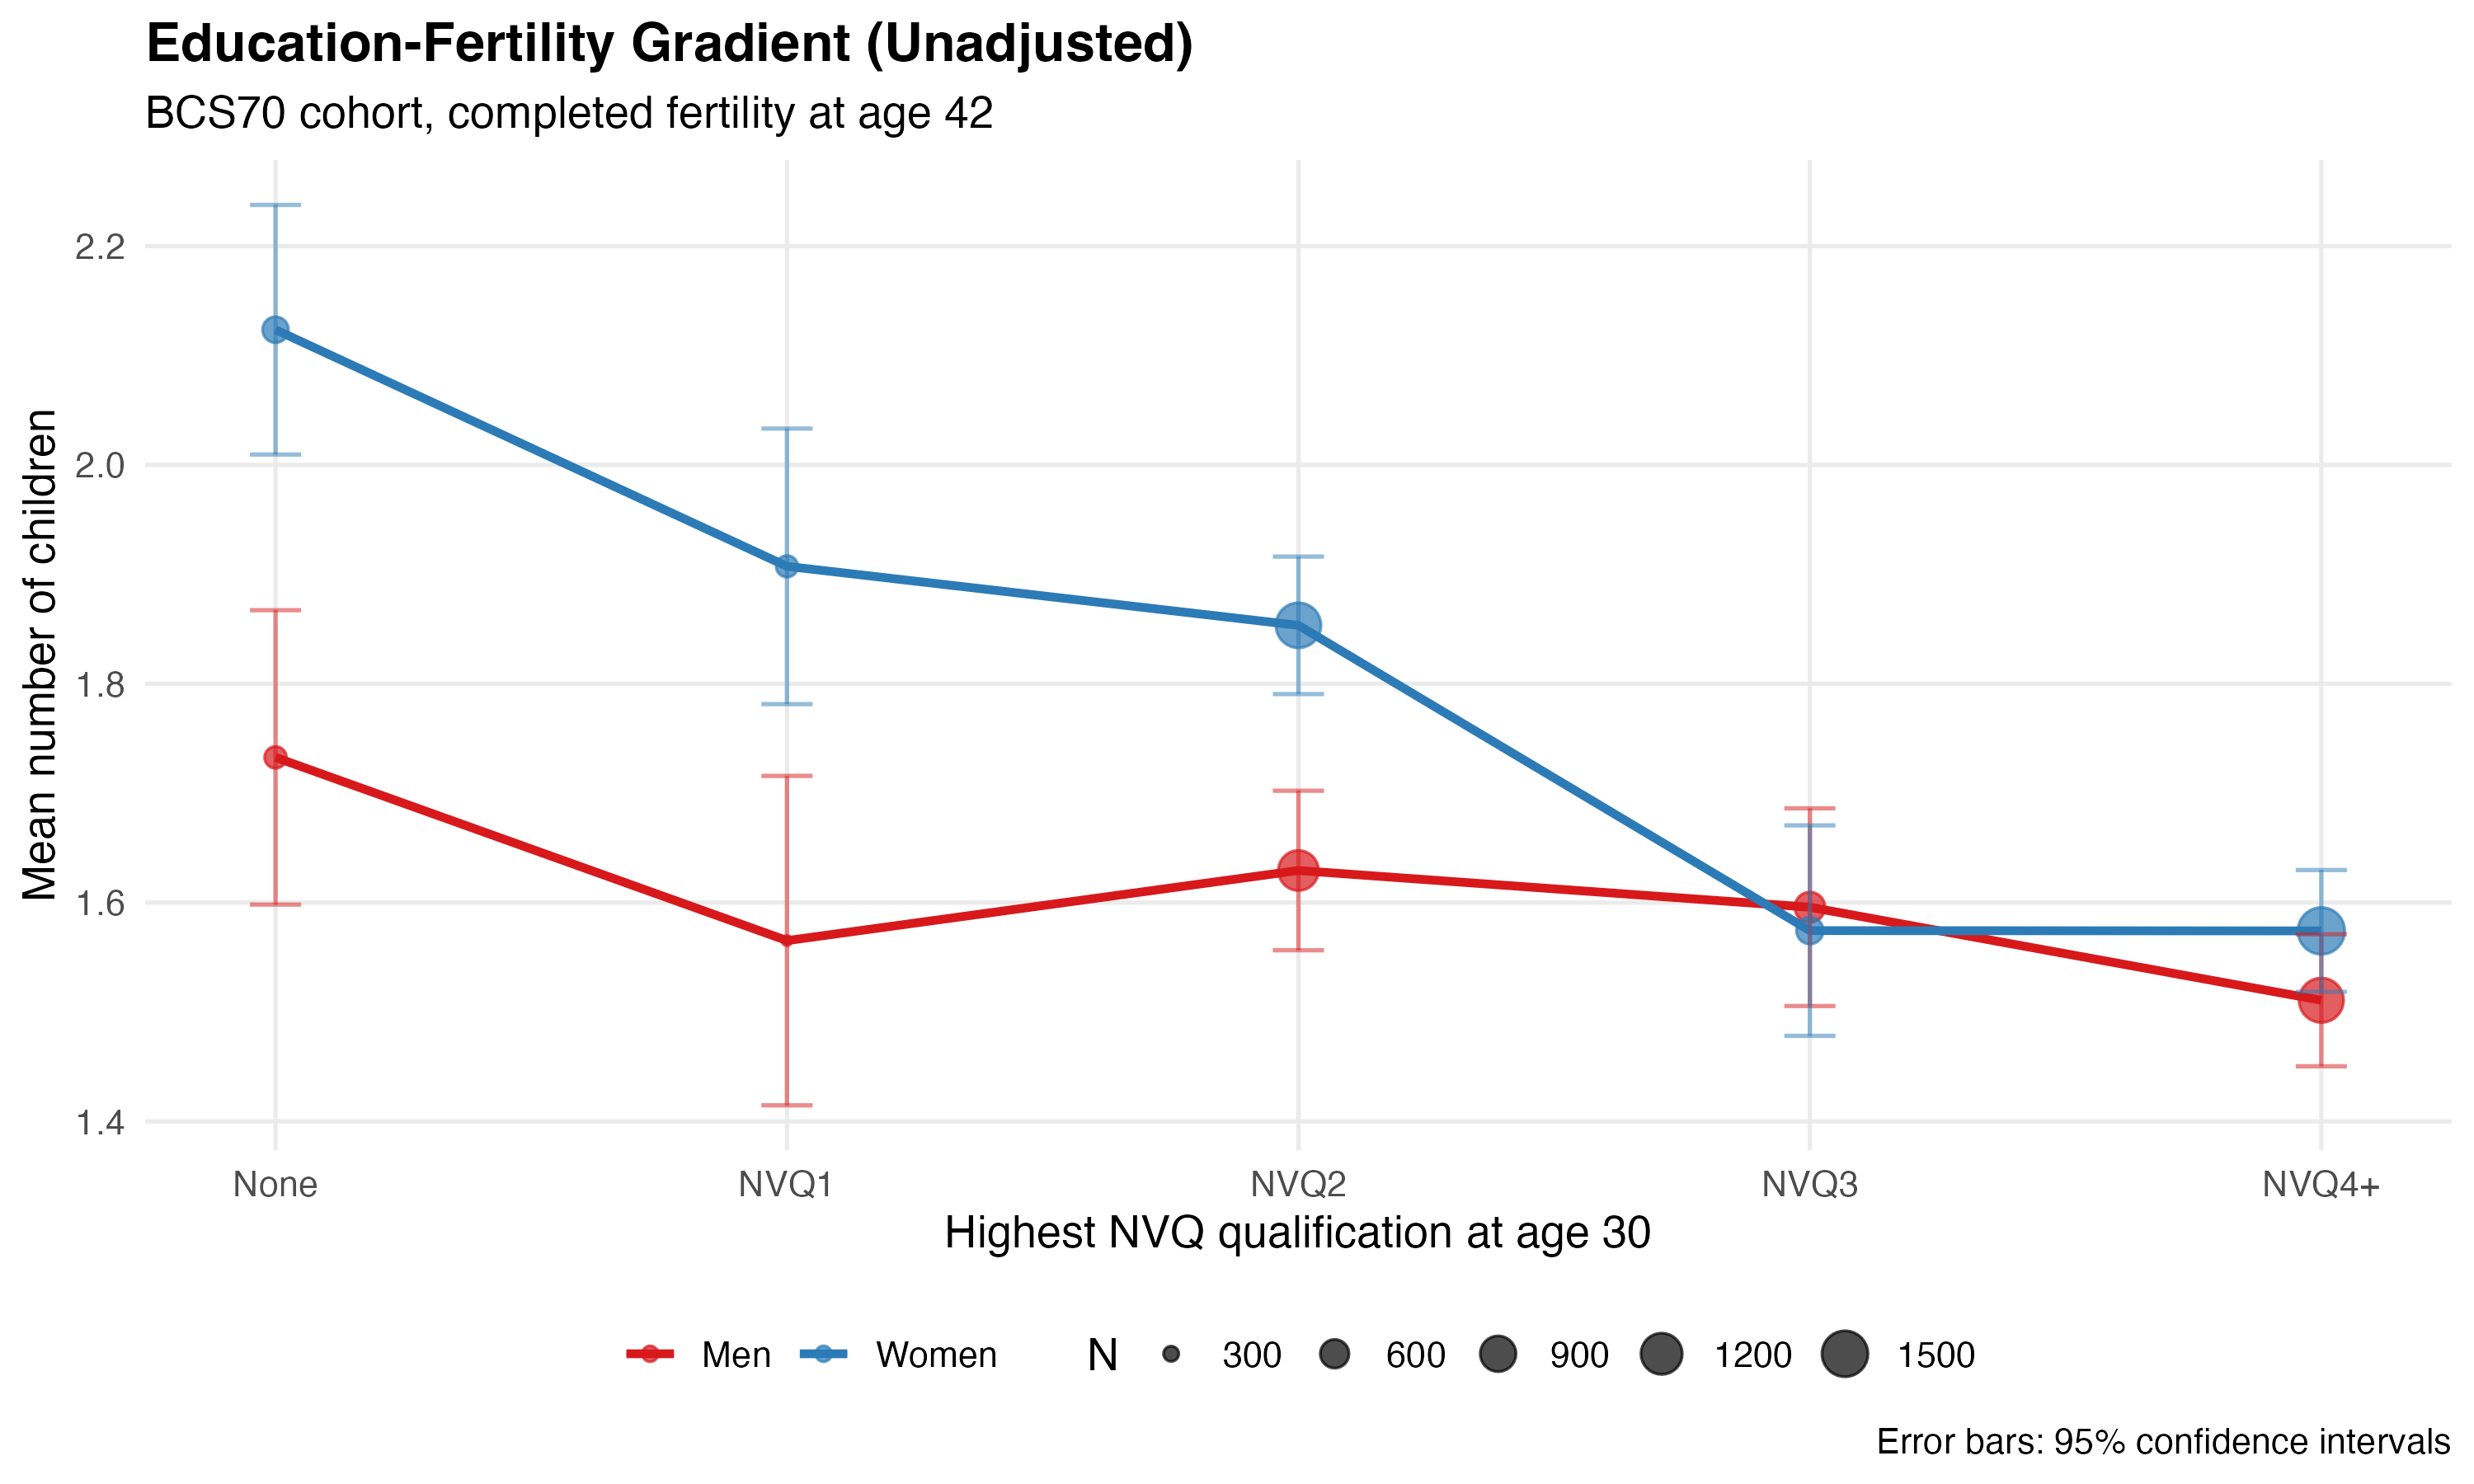
\includegraphics[width=0.8\textwidth]{h4_raw_gradient.png}
\caption{Unadjusted education--fertility gradient in BCS70 by sex. Mean completed fertility at age 42 by highest NVQ qualification at age 30; error bars are 95\% confidence intervals.}
\label{fig:rawgrad}
\end{figure}

\begin{figure}[ht]
\centering

\includegraphics[width=0.8\textwidth]{h4_dml_total_effects.png}
\caption{H4, DML estimates of the total causal effect of education on completed fertility, with 95\% confidence intervals. Estimation samples ($N=1{,}461$ women, $1{,}081$ men) reflect complete cases on all pre-treatment confounders. The women's estimate is significant; the men's is not distinguishable from zero.}
\label{fig:dmltotal}
\end{figure}

\section{H4: sequential mediation and pathway decomposition}
\label{sec:h4med}
Running the DML procedure four times, sequentially adding mediator blocks (Table~\ref{tab:seq}), is
informative for women. The estimate barely moves from M0 to M1 ($-0.133$ to $-0.130$): the attitudinal
mediators absorb only about 2\% of the total effect. The largest drop is from M1 to M2 ($-0.130$ to
$-0.049$, with significance lost at $p=0.118$): earnings absorb by far the largest share. Adding
partnership at M3 produces a partial reversal (to $-0.082$, $p=0.017$), implying that partnership
operates opposite to earnings. For men the pattern is suppression rather than mediation: the estimate
becomes more negative with each block, from $-0.047$ to $-0.091$, and attains conventional
significance only once mediators are conditioned on.

\begin{table}[ht]
\centering
\caption{H4, sequential mediation decomposition by sex; declining $N$ reflects complete-case attrition.}
\label{tab:seq}
\small
\begin{tabular}{@{}llccc@{}}
\toprule
Stage & Mediators added & $N$ & $\theta$ (SE) & $p$ \\
\midrule
M0 (women) & None (total effect) & 1{,}461 & $-0.133$ (0.028) & $<0.001$ \\
M1 (women) & + Attitudinal & 1{,}453 & $-0.130$ (0.028) & $<0.001$ \\
M2 (women) & + Earnings & 1{,}046 & $-0.049$ (0.031) & 0.118 \\
M3 (women) & + Partnership & 812 & $-0.082$ (0.034) & 0.017 \\
M0 (men)   & None (total effect) & 1{,}081 & $-0.047$ (0.033) & 0.148 \\
M1 (men)   & + Attitudinal & 1{,}075 & $-0.067$ (0.033) & 0.045 \\
M2 (men)   & + Earnings & 827 & $-0.094$ (0.039) & 0.016 \\
M3 (men)   & + Partnership & 678 & $-0.091$ (0.042) & 0.029 \\
\bottomrule
\end{tabular}
\end{table}

Table~\ref{tab:pathway} reports the pathway shares. For women, the economic pathway accounts for
61.2\% of the total effect, the attitudinal pathway for 2.2\%, the partnership pathway for
$-25.0\%$ (operating in the opposite direction, consistent with highly educated women being more
likely to be partnered at age 42), and the direct effect for 61.6\%. For men the direct effect
($-0.091$) exceeds the total ($-0.047$), the 193\% figure, reflecting suppression by the economic
mediator rather than mediation. Because the men's total effect is not statistically distinguishable
from zero ($p=0.148$), the percentage shares for men are not meaningfully interpretable and are
reported for completeness only. The conclusion is contrary to H4: the individual-level
education--fertility relationship, in this cohort, is mediated by economic rather than
attitudinal pathways, consistent with the quantity--quality framework of \citet{becker1960}
and \citet{kaplan1996} and inconsistent with the strong individual-level reading of cultural
transmission \citep{bongaartswatkins1996,colleran2016}. Three caveats temper the verdict. First, the
earnings mediator is measured at age~42, contemporaneous with the outcome, so reverse causality is not
merely possible but is the central finding of the motherhood-wage-penalty literature. The economic
pathway of $-0.081$ therefore includes both education~$\to$~earnings~$\to$~fertility \emph{and} the
reverse channel, making it an upper bound that overstates the economic contribution. Second, the
attitudinal mediators are measured at age~30, contemporaneous with the treatment, so the
attitudinal pathway may be understated. Third, the result generalises only to
similar cohorts in similar settings.

A fourth concern is more serious, because it bears on the headline share directly: because sample size
declines as mediators enter, each difference in Table~\ref{tab:seq} combines mediation with a change in
who is in the estimation sample. The largest drop, from M1 to M2, coincides with the loss of 407 women,
and those women are disproportionately lower-educated and higher-parity (Section~3.4), so deleting them
mechanically flattens the education--fertility slope. Table~\ref{tab:common} re-estimates all four
stages on the single common sample of $N=812$ that satisfies every mediator simultaneously, which holds
composition fixed. The total effect there is $-0.108$ ($p=0.002$), against $-0.133$ on the full
complete-case sample: roughly a fifth of the effect magnitude is compositional, and four-fifths is not.
The causal claim therefore survives, but the pathway shares shift. Holding composition fixed, the
economic pathway accounts for 44.3\% of the total effect rather than 61.2\%, the partnership pathway
for $-12.0\%$, and the attitudinal pathway for $-8.1\%$: attitudes now work weakly \emph{against} the
total effect rather than mediating it. The honest summary is that the economic share lies in the
mid-forties once composition is held fixed, with 61.2\% an upper bound for the two distinct reasons of
reverse causality and selective attrition. What does not change under either specification is the
ordering: the attitudinal pathway is negligible, and its sign is not even stable across
specifications, which is a stronger falsification of H4 than a small positive share would have been.

\begin{table}[ht]
\centering
\caption{H4 robustness, mediator sequence re-estimated on the common sample of women complete on all mediators ($N=812$ at every stage), compared with the sequential estimates of Table~\ref{tab:seq}.}
\label{tab:common}
\small
\begin{tabular}{@{}lcccc@{}}
\toprule
Stage & Sequential $\theta$ & Sequential $N$ & Common-sample $\theta$ (SE) & $p$ \\
\midrule
M0 (total)      & $-0.133$ & 1{,}461 & $-0.108$ (0.035) & 0.002 \\
M1 (+attitudes) & $-0.130$ & 1{,}453 & $-0.116$ (0.035) & 0.001 \\
M2 (+earnings)  & $-0.049$ & 1{,}046 & $-0.069$ (0.035) & 0.050 \\
M3 (+partnership) & $-0.082$ & 812 & $-0.082$ (0.034) & 0.017 \\
\midrule
\multicolumn{5}{@{}l}{\footnotesize Common-sample pathway shares: attitudinal $-8.1\%$, economic 44.3\%, partnership $-12.0\%$, direct 75.9\%.} \\
\bottomrule
\end{tabular}
\end{table}

\begin{table}[ht]
\centering
\caption{H4, pathway decomposition by sex. Indirect effects by subtraction; the direct effect is the residual. Shares can exceed 100\% when pathways oppose.}
\label{tab:pathway}
\small
\begin{tabular}{@{}lcccc@{}}
\toprule
Pathway & Women (effect) & Women (\% total) & Men (effect) & Men (\% total) \\
\midrule
Attitudinal        & $-0.003$ & 2.2\% & $+0.019$ & $-40.7\%$ \\
Economic (earnings) & $-0.081$ & 61.2\% & $+0.027$ & $-57.1\%$ \\
Partnership        & $+0.033$ & $-25.0\%$ & $-0.002$ & 5.0\% \\
Direct (residual)  & $-0.082$ & 61.6\% & $-0.091$ & 192.8\% \\
\bottomrule
\end{tabular}
\end{table}

\begin{figure}[ht]
\centering

\includegraphics[width=0.8\textwidth]{h4_dml_mediation_waterfall.png}
\caption{H4, mediation decomposition for women and men. Bars show the indirect effect through each pathway and the controlled direct effect; percentages are the pathway share of the total effect.}
\label{fig:waterfall}
\end{figure}

\section{Synthesis}
Read together, the H3 and H4 findings point consistently away from cultural transmission as the
proximate individual mechanism. At the country level the cultural and economic blocks cannot be
separated at $N=21$, though the economic block holds the narrow inferential edge. At the individual
level the verdict is sharper: earnings account for between 44\% and 61\% of the education effect on
women's fertility, depending on whether sample composition is held fixed, while the attitudinal pathway
is negligible under either specification. Together with the U-shape findings, this
discriminates the frameworks: the quantity--quality and opportunity-cost accounts receive the most
support, cultural transmission is contradicted at the individual level while retaining mixed support at
the country level, and the maladaptation framework, though not directly tested, sits less comfortably
with an opportunity-cost mechanism than the rational-choice account does. Whether cultural transmission
might still operate as a population-level propagation mechanism without being the dominant individual
mediator is taken up in Chapter~7.

% ==========================================================================
% CHAPTER 7
% ==========================================================================
\chapter{Discussion}

The empirical chapters produced four findings whose implications now require integration: the
European gradient is non-monotonic, with medium-educated women lowest; cross-country variation cannot
be definitively attributed to cultural or economic characteristics at $N=21$, though the economic
block holds a narrow edge; the individual education effect on women's fertility is mediated primarily
by earnings, contradicting H4; and the U-shape, robust across countries, is not robust to population
weighting. This chapter situates these in the literature, draws out their theoretical implications,
acknowledges limitations, and identifies directions for future work.

\section{Theoretical implications}
Stated in one sentence, the contribution is this: the contemporary European education--fertility
gradient is not a monotonic relationship in completed quantity but a U-shape in level combined with a
tempo effect concentrated in the early twenties, and the individual-level mechanism that produces it is
economic rather than attitudinal.

The first implication is descriptive: the gradient is dominantly U-shaped, with medium-educated women
at the bottom in fourteen of twenty-one countries, so the classical framing in which fertility falls
monotonically with resources is too simple. The \citet{stulpbarrett2016} review identified the J-curve as
theoretically important but empirically fragmentary; the contribution here is not merely that
non-monotonicity exists but that the U-shape is the dominant pattern.

The second concerns cultural transmission, which predicts both that norms
propagate through populations via social transmission and that the proximate mechanism by which
education depresses individual fertility is attitudinal change. The H4 result contradicts the
proximate-mechanism claim, and at the country level the cultural block does not dominate. Yet this does
not refute the framework: cultural transmission may be right about long-run population-level
propagation while being wrong about the short-run translation of individual education into individual
fertility, which is what my evidence speaks to.

The third concerns the paradox itself. \citet{vining1986} framed it as a uniform negative gradient;
my findings refine it in two ways. First, the negative gradient is real at the low--high comparison
but its bottom sits at medium education. Second, that gradient is a phenomenon of timing, located
in ages 20--24 and reversing over ages 25--49 (Section~\ref{sec:agefloor}). Read alongside the H4
result these cohere: opportunity cost is intrinsically a claim about timing, biting hardest when
earnings and childbearing compete most directly, so a macro gradient concentrated in the early
twenties and a micro mechanism running through earnings are the same phenomenon at two
scales. Under quantity--quality the U-shape is then expected if medium-educated women
face the steepest opportunity costs, with meaningful wage penalties but insufficient earnings to
outsource childcare. That remains speculative, since this dissertation
does not test whether earnings mediation is strongest for medium-educated women specifically. The
maladaptation framework \citep{perusse1993,kanazawa2003} is not directly tested, but the dominance of
realised opportunity cost over evolved attitudes shifts the burden toward accounts with
rational economic responses as their proximate mechanism.

\section{Comparison with prior literature}
The H4 finding is best read against \citet{snopkowski2016}, whose multi-site SEM analysis found that
education retains a direct effect on fertility, beyond both economic and cultural-transmission
mediators, in two of its three sites. The authors leave that residual open, attributing it to
horizontal cultural transmission or to unobserved contextual characteristics. Their sites were rural,
kin-dense contexts in which women's labour integrates with childcare and allocare from kin buffers the
opportunity cost of work, conditions the authors explicitly contrast with long-industrialised
societies and urban areas; BCS70 samples exactly such an industrialised setting. That the economic
pathway dominates here is consistent with opportunity-cost mechanisms operating most strongly where
the earlier study could not observe them, and suggests the unattributed residual in industrialised
contexts may itself be economic rather than attitudinal. \citet{jalovaara2019} raise the complementary
challenge from the other direction, cautioning that highly educated women need not face the higher
opportunity costs the literature assumes, since Nordic childcare and parental-leave provision may
leave them facing lower costs than the less educated. Both points converge on the same conditional:
opportunity cost dominates where institutions do not buffer it, which describes the British setting
BCS70 samples more closely than the Nordic one. The analysis also provides the
causal-mediation complement to
\citet{berrington2017}'s descriptive work on intention--realisation divergence in this cohort. The
positive partnership pathway is consistent with partnered status raising
fertility; highly educated women in BCS70 are more likely to be partnered at age~42, so partnership
partially offsets the negative earnings channel.

\section{Strengths and limitations}
The strategy's strengths are the application of double machine learning \citep{chernozhukov2018} to
BCS70, to my knowledge the first DML mediation decomposition on this cohort's age-30 to age-42
sweeps; the staged discovery--inference design for H3 that treats the SHAP--WAIC disagreement as a
finding rather than a problem; and the combination of fixed-effects, quadratic, and quantile methods
for H1 and H2 with a robustness battery that exposes the U-shape's sensitivity to population weighting.

The most consequential limitation is the pivot from completed cohort
fertility to period eTFR, which conflates the tempo and quantum of fertility
\citep{bongaartsfeeney1998,kohlerphilipov2001}: Section~\ref{sec:agefloor} shows the sign of the H1
contrast depends on the age range over which the eTFR is cumulated, and Section~6.3 notes that the H3
outcome inherits the same problem. Tempo-adjusted measures require parity-specific mean ages at birth
the Eurostat series does not supply. The findings therefore describe the European period regime over
2007--2024 rather than the lifetime fertility of any cohort. The country sample of $N=21$ (18 in the
Bayesian common case) is the binding constraint on H3: no comparison produces intervals that cleanly
exclude zero, and the LOOCV $R^2$ of $-0.086$ shows the feature importances do not generalise. Several
economic predictors the literature treats as important, among them childcare costs, housing
affordability and welfare generosity, could not be included on a consistent panel basis, so the economic
block is operationalised narrowly and its modest WAIC advantage may understate the economic
contribution. The H3 outcome also averages each country's gradient over its own coverage window, so the
resulting period confound cannot be separated from cross-country variation at this sample size.

The H4 analysis rests on a single British 1970 cohort. Its most consequential limitation, developed in
Section~\ref{sec:h4med}, is the contemporaneous measurement of earnings and fertility at age~42: the
motherhood wage penalty makes the $-0.081$ economic indirect effect an upper bound, so the 61.2\%
sequential share is a ceiling. With composition held fixed the share is 44.3\%, so the defensible
statement is that the economic pathway accounts for between two-fifths and three-fifths of the effect;
the ordering is unaffected either way. The attitudinal mediators are measured at age~30, contemporaneous
with the treatment, making sequential ignorability \citep{imai2010} harder to defend, and the
partnership mediator functions as an additional confounder rather than a downstream mediator. The
U-shape is not robust to population weighting, so it characterises European countries as units more
than European women as a population.

Attrition in BCS70 is non-random with respect to education, and the analytical sample of $N=8{,}318$ is
approximately half the original birth cohort, 85\% of the 9{,}840 observed at the age-42 sweep. On the
observable part of this problem the common-sample re-estimation is informative: holding the estimation
sample fixed reduces the total effect from $-0.133$ to $-0.108$, so selection on the variables driving
the mediator cascade accounts for roughly a fifth of the effect magnitude, not for the effect itself.
Selection on unobservables remains possible, and inverse-probability-of-attrition weighting
\citep{hernan2004} would be the appropriate remedy.

Several smaller constraints remain. The wild-cluster bootstrap recommended at 21 clusters
\citep{cameron2008} could not be run, but the CR2 estimator (Section~\ref{sec:cr2}) addresses the same
concern; the quantile regressions are identified only in the central portion of the distribution; the
12\% classification threshold is empirical rather than theoretical; the \texttt{post\_socialist}
indicator collapses heterogeneity in pronatalist-policy histories; and ESS coverage is incomplete.

\section{Future research}
Five directions follow. Replicating the H4 analysis in the 1958 NCDS or comparable panels would test
whether earnings dominance is stable across cohorts and settings. Recomputing gradient steepness on a
25--49 basis and refitting the H3 models would establish whether the country-level results are
themselves tempo artefacts. Extending H3 to a larger country sample, with childcare-cost and housing
indicators added, would lift the Bayesian comparison out of the zero-crossing regime. Modelling BCS70
partnership histories longitudinally rather than as an age-42 snapshot would decompose the partnership
pathway into selection and exposure, and adding partner-level earnings would identify the
assortative-mating channel central to quantity--quality. Finally, testing the macro--micro
reconciliation directly, by combining cohort data with measures of attitudinal diffusion, would address
how individual economic responses and population-level cultural transmission jointly produce observed
patterns.

% ==========================================================================
% CHAPTER 8
% ==========================================================================
\chapter{Conclusion}

This dissertation asked what shape the education--fertility gradient takes across European populations
in 2007--2024, and what predicts its steepness, its shape, and the individual mechanism through which it
operates. H1 was supported in the baseline specification: the high--low contrast
in log eTFR is $-0.187$ ($p=0.002$) across the 21-country panel, robust to the four conventional
sensitivity checks, but not to the age range over which the rate is cumulated:
restricting the eTFR to ages 25--49 reverses its sign to $+0.201$ ($p=0.002$), locating the
conventional gradient in ages 20--24 and identifying it as a phenomenon of fertility timing rather
than of completed family size. H2 was supported
parametrically and distributionally, with the U-shape the dominant gradient type across 14 of 21
countries, the quadratic minimum between the medium and high tiers (educ $=1.24$), and
medium-educated women lowest at every age floor tested. H3 was unsupported
in the strong sense: at $N=21$ neither block produces a definitive ranking, and the LOOCV $R^2$ of
$-0.086$ shows macro indicators lack reliable out-of-sample predictive power. H4 was contradicted: for
women, earnings account for between two-fifths and three-fifths of the
total effect depending on whether sample composition is held fixed, while the attitudinal pathway is
negligible under either specification and its sign is not stable across them.

Three contributions follow. The first is the systematic cross-country documentation of the U-shape as
the dominant gradient type in contemporary Europe, filling the gap the \citet{stulpbarrett2016} review
identified. The second is the application of double machine learning causal mediation to BCS70, whose
finding that the economic pathway dominates constrains the cultural-transmission account at the
individual level. The third is the discovery--inference pipeline for H3 and the honest treatment of the
disagreement between its stages, in a literature where small-sample cross-country regressions are too
often reported with more confidence than the data warrant.

Theoretically, the gradient is non-monotonic at the population level; cultural transmission
in its strong individual-level reading receives less support than the literature has assumed, though a
weaker population-propagation reading remains tenable; and the paradox is more limited and more
economically rational at the proximate level than \citet{vining1986}'s original framing implied. Whether
the opportunity-cost responses that depress contemporary fertility are nonetheless maladaptive
over multigenerational fitness is a question this single-generation evidence cannot resolve, though the
\citet{goodman2012} finding suggests the answer may be yes.

% ==========================================================================
% APPENDICES
% ==========================================================================
\appendix

\chapter{Full 21-Country Gradient Steepness Table}

Table~\ref{tab:appA} reports, for each of the 21 countries, mean period eTFR by education tier
across 2007--2024, the gradient steepness (low minus high), the share of women aged 25--39 in the
low-education tier, and the gradient-shape classification. Countries are ordered by steepness.

\begin{table}[ht]
\centering
\caption{Mean eTFR by tier, gradient steepness, low-tier share, and shape classification, 21 European countries, each over its coverage window within 2007--2024.}
\label{tab:appA}
\small
\begin{tabular}{@{}lcccccl@{}}
\toprule
Country & Low & Medium & High & Steepness & Low share (\%) & Shape \\
\midrule
Slovakia        & 2.79 & 1.24 & 1.47 & $+1.32$ & 6.6  & U-shape (composition) \\
Latvia          & 2.10 & 1.27 & 1.40 & $+0.70$ & 7.5  & U-shape (composition) \\
Türkiye         & 2.17 & 1.85 & 1.50 & $+0.67$ & 56.4 & Monotonic negative \\
Spain           & 1.49 & 1.28 & 0.86 & $+0.63$ & 30.5 & Monotonic negative \\
Slovenia        & 2.26 & 1.34 & 1.65 & $+0.61$ & 6.0  & U-shape (composition) \\
Greece          & 1.87 & 1.24 & 1.27 & $+0.60$ & 15.2 & U-shape (broad) \\
North Macedonia & 2.15 & 1.16 & 1.56 & $+0.59$ & 30.3 & U-shape (broad) \\
Finland         & 2.23 & 1.38 & 1.64 & $+0.58$ & 7.5  & U-shape (composition) \\
Estonia         & 1.91 & 1.47 & 1.50 & $+0.41$ & 8.9  & U-shape (composition) \\
Sweden          & 2.03 & 1.75 & 1.65 & $+0.38$ & 10.8 & Monotonic negative \\
Czechia         & 1.83 & 1.32 & 1.47 & $+0.36$ & 6.2  & U-shape (composition) \\
Hungary         & 1.66 & 1.21 & 1.36 & $+0.30$ & 13.6 & U-shape (broad) \\
Austria         & 1.43 & 1.33 & 1.19 & $+0.24$ & 15.6 & Monotonic negative \\
Portugal        & 1.54 & 1.33 & 1.30 & $+0.24$ & 33.1 & Monotonic negative \\
Croatia         & 1.68 & 1.44 & 1.53 & $+0.15$ & 8.6  & U-shape (composition) \\
Serbia          & 1.77 & 1.34 & 1.67 & $+0.10$ & 12.8 & U-shape (broad) \\
Belgium         & 1.57 & 1.61 & 1.56 & $+0.01$ & 17.4 & Inverted bottom \\
Romania         & 1.91 & 1.15 & 1.91 & $+0.00$ & 21.6 & U-shape (broad) \\
Norway          & 1.65 & 1.34 & 1.73 & $-0.08$ & 14.8 & U-shape (broad) \\
Poland          & 1.26 & 1.25 & 1.39 & $-0.13$ & 4.8  & U-shape (composition) \\
Denmark         & 1.31 & 1.47 & 1.78 & $-0.46$ & 15.9 & Inverted bottom \\
\bottomrule
\end{tabular}
\end{table}

\noindent Three countries record negative steepness, high-educated women above low-educated:
Denmark decisively, Norway and Poland marginally. Poland's classification as a U-shape
rests on a low--medium difference of 0.01 eTFR, and Greece's and Estonia's on medium--high
differences of 0.03; these sit within measurement-error margins and are discussed in
Section~\ref{sec:shape}.

\chapter{Full Robustness Checks}

This appendix reports supplementary diagnostics supporting Chapters~5 and~6: the evidence on age
composition underlying the age-floor analysis of Section~\ref{sec:agefloor}, and two H3 diagnostics.

\section*{Age-floor diagnostics}

Table~\ref{tab:appB1} reports the educational composition of women by age group, averaged across all
country--years. It is the evidence that adjudicates between an artefactual and a substantive reading
of the age-floor reversal. At ages 15--19 the low tier holds 82\% of women and the high tier is
empty, because upper secondary is not yet complete and a tertiary qualification is unattainable at
that age: the classification there is mechanical rather than behavioural. At ages 20--24, by
contrast, the low tier holds 14.0\% of women, almost exactly the 13.8\% observed at 25--29, so the
low tier at the ages that drive the reversal is not mechanically inflated.

\begin{table}[ht]
\centering
\caption{Educational composition of women by age group. Mean percentage in each tier across all country--years, 21 countries, 2007--2024.}
\label{tab:appB1}
\begin{tabular}{@{}lccc@{}}
\toprule
Age group & Low (\%) & Medium (\%) & High (\%) \\
\midrule
15--19 & 82.0 & 18.0 & 0.0 \\
20--24 & 14.0 & 70.8 & 15.2 \\
25--29 & 13.8 & 44.0 & 42.2 \\
30--34 & 15.4 & 42.4 & 42.3 \\
35--39 & 18.2 & 45.6 & 36.2 \\
40--44 & 18.2 & 45.6 & 36.2 \\
45--49 & 24.3 & 48.3 & 27.4 \\
\bottomrule
\end{tabular}

\vspace{0.5em}
\parbox{0.85\textwidth}{\footnotesize The 35--39 and 40--44 rows are identical because
\texttt{edat\_lfse\_03} reports attainment for a single 35--44 band, whose shares are applied to both
five-year subgroups. This is the uniform-attainment assumption described in
Section~\ref{sec:etfr}, and it is defensible at these ages, where attainment has long stabilised.}
\end{table}

Table~\ref{tab:appB2} decomposes each tier's eTFR by age group, showing where each tier's fertility
is located across the reproductive span. Low-educated women draw 38.2\% of their eTFR from ages
15--24 against 11.9\% for high-educated women, and the modal contribution occurs at 20--24 for the
low tier but 30--34 for the high tier. This is the tempo difference that drives the H1 reversal.

\begin{table}[ht]
\centering
\caption{Contribution to eTFR by age group and education tier, as a percentage of that tier's total. Computed as $5\times$ mean ASFR in each cell, pooled across 21 countries and 2007--2024.}
\label{tab:appB2}
\begin{tabular}{@{}lccccccc@{}}
\toprule
Tier & 15--19 & 20--24 & 25--29 & 30--34 & 35--39 & 40--44 & 45--49 \\
\midrule
Low    & 3.2 & \textbf{35.0} & 30.3 & 19.8 & 9.2  & 2.3 & 0.1 \\
Medium & 5.5 & 13.3 & \textbf{34.7} & 29.7 & 13.7 & 3.0 & 0.2 \\
High   & 0.2 & 9.9  & 27.0 & \textbf{37.2} & 21.4 & 4.0 & 0.4 \\
\bottomrule
\end{tabular}

\vspace{0.5em}
\parbox{0.85\textwidth}{\footnotesize Bold entries mark each tier's modal age group. Share of eTFR
originating before age 25: low 38.2\%, medium 18.8\%, high 11.9\%.}
\end{table}

\section*{H3 diagnostics}

Two supplementary H3 diagnostics follow: the predictor correlation matrix
(Figure~\ref{fig:corr}), which motivates the decision to include at most two V-Dem indices in any
Bayesian model, and the SHAP dependence plot for the leading predictors (Figure~\ref{fig:shapdep}).

\begin{figure}[ht]
\centering

\includegraphics[width=0.8\textwidth]{h3_correlation_matrix.png}
\caption{Correlation matrix of the twelve country-level predictors used in the H3 analysis.}
\label{fig:corr}
\end{figure}

\begin{figure}[ht]
\centering

\includegraphics[width=0.8\textwidth]{h3_shap_dependence.png}
\caption{SHAP dependence for the leading H3 predictors, showing how each feature's contribution varies with its value.}
\label{fig:shapdep}
\end{figure}

\chapter{Code and Reproduction Information}

All analyses were conducted in R~4.5.1. The analysis pipeline comprises the following numbered
scripts, executed sequentially:

\begin{description}
\item[\texttt{00\_setup\_project.R}] Creates the project directory structure and function-file stubs.
\item[\texttt{01\_inspect\_data.R}] Inspects the raw Eurostat and Wittgenstein source files prior to cleaning.
\item[\texttt{01\_clean\_eurostat.R}] Filters the Eurostat fertility and attainment extracts to the country, age-group, and ISCED categories used in the analysis.
\item[\texttt{02\_descriptive\_dataset1.R}] Builds Dataset~1: education-specific ASFRs from \texttt{demo\_faeduc}, \texttt{edat\_lfse\_03}, and \texttt{demo\_pjangroup}, and aggregates them to the period eTFR panel.
\item[\texttt{02b\_gradient\_shape.R}] Classifies the 21 countries by gradient shape using the mean eTFR ordering and the low-tier population share.
\item[\texttt{03\_h1\_models.R}] Estimates the H1 two-way fixed-effects models, the country~$\times$~education interactions, and the robustness battery.
\item[\texttt{04\_h2\_models.R}] Estimates the H2 quadratic specification and the quantile regressions.
\item[\texttt{05\_dataset2\_outcomes.R}] Derives the country-level gradient outcomes (steepness, U-shape indicator) from Dataset~1.
\item[\texttt{06\_dataset2\_predictors.R}] Assembles the V-Dem, OECD, and World Bank country-level predictors.
\item[\texttt{06b\_ess\_cultural\_predictors.R}] Extracts eight ESS core-module items and aggregates them into the three attitudinal composites.
\item[\texttt{07\_h3\_models.R}] Fits the XGBoost Stage~1 model with SHAP decomposition and the six Stage~2 Bayesian models via \texttt{brms}.
\item[\texttt{08\_h4data\_bcs70.R}] Reads and harmonises the BCS70 sweep files; constructs treatment, outcome, confounder, and mediator variables.
\item[\texttt{08\_h4dml\_bcs70.R}] Estimates the DML total effects and the sequential mediation decomposition.
\item[\texttt{09\_robustness\_age2549.R}] Rebuilds the eTFR panel over ages 25--49 and re-runs the H1, H2, and shape-classification tests as a robustness check on the uniform-attainment assumption.
\item[\texttt{10\_diagnostic\_agefloor.R}] Sweeps the eTFR age floor across 15, 20, and 25; decomposes each tier's eTFR by age group and reports the education composition of women by age group.
\item[\texttt{11\_h2\_quantile\_bootstrap.R}] Re-runs the H2 quantile regressions with country-clustered bootstrap standard errors.
\item[\texttt{12\_h1\_cr2\_clubsandwich.R}] Re-estimates the H1 battery with CR2 bias-reduced cluster-robust standard errors and Satterthwaite degrees of freedom.
\end{description}

\noindent Three auxiliary scripts support verification rather than estimation:
\texttt{data\_check.R} prints the structure of all three analytical datasets;
\texttt{audit\_chapter3.R} extracts reported figures from the saved model objects for cross-checking against the text; and
\texttt{robustness\_check.R} re-runs the population-weighted specification in isolation.

\noindent Key R packages and versions: \texttt{fixest} (panel regression), \texttt{quantreg}
(quantile regression), \texttt{xgboost} (gradient boosting), \texttt{brms} (Bayesian regression),
\texttt{DoubleML} (double machine learning), \texttt{ranger} (random forests), \texttt{haven}
(Stata file reading).

\noindent\textbf{Code availability.} The complete analysis pipeline, including all scripts listed
above, is publicly available at
\url{https://github.com/RoudraSarkar/demographic-transition-fitness-paradox}.

\noindent\textbf{Data access.} Eurostat, V-Dem, OECD, and World Bank data are freely downloadable.
The ESS integrated file requires free registration at
\url{https://www.europeansocialsurvey.org}. BCS70 data are available under standard academic
licence via the UK Data Service (\url{https://ukdataservice.ac.uk}); studies used are
UKDA-SN-2666, 3535, 3723, 5558, 6095, 7473, and 9347.

% ==========================================================================
% BIBLIOGRAPHY
% ==========================================================================
\bibliography{references}

\end{document}
